% ============================================================
%  PE2 -- Práctica Experimental | Unidad 2
%  Elicitación y Análisis de Requisitos
%  Asignatura: Ingeniería de Requisitos (ISR-401) -- UTEQ 2026-2027
%  Sistema del PFC: MundiPets
%  Formato: IEEE onecolumn | Biber + biblatex (estilo IEEE)
% ============================================================
\documentclass[journal,onecolumn]{IEEEtran}

% ── Codificación e idioma ───────────────────────────────────
\usepackage[T1]{fontenc}
\usepackage[utf8]{inputenc}
\usepackage[spanish, es-tabla]{babel}
\usepackage[autostyle=true, spanish=mexican]{csquotes}

% ── Tablas ──────────────────────────────────────────────────
\usepackage{booktabs}
\usepackage{tabularx}
\usepackage{array}
\usepackage{multirow}
\usepackage{longtable}

% ── Figuras ─────────────────────────────────────────────────
\usepackage{graphicx}
\usepackage{float}

% ── Color y enlaces ─────────────────────────────────────────
\usepackage{xcolor}

% ── Geometría ───────────────────────────────────────────────
\usepackage{geometry}
\geometry{a4paper, top=2.5cm, bottom=2.5cm, left=2.5cm, right=2.5cm}

% ── Encabezado ──────────────────────────────────────────────
\usepackage{fancyhdr}
\pagestyle{fancy}
\fancyhf{}
\renewcommand{\headrulewidth}{0.4pt}
\fancyhead[L]{\small PE2 -- Unidad 2 | Ingeniería de Requisitos}
\fancyhead[R]{\small MundiPets -- Elicitación y Análisis de Requisitos}
\fancyfoot[C]{\thepage}

% ── Espaciado ───────────────────────────────────────────────
\usepackage{parskip}
\setlength{\parskip}{4pt}
\makeatletter
\@ifundefined{labelindent}{}{\let\labelindent\relax}
\makeatother
\usepackage{enumitem}
\usepackage{caption}
\usepackage{titlesec}
\captionsetup{font=small, labelfont=bf}
\usepackage{amssymb}

% ── Forzar "Tabla" en lugar de "Cuadro" ──────────────────────
\renewcommand{\thetable}{\arabic{table}}
\def\tablename{Tabla}

% ── Caja de guía (fondo gris claro, borde negro) ─────────────
\usepackage{mdframed}
\mdfdefinestyle{guia}{
  linecolor=black,
  linewidth=0.6pt,
  backgroundcolor=gray!10,
  innertopmargin=6pt,
  innerbottommargin=6pt,
  innerleftmargin=8pt,
  innerrightmargin=8pt,
  skipabove=4pt,
  skipbelow=4pt
}

% ── Comando de caja de guía (Responsable) ────────────────────
\newcommand{\guia}[2]{%
  \begin{mdframed}[style=guia]
    \noindent\textbf{Responsable: #1}\\[2pt]
    #2
  \end{mdframed}
}

\renewcommand{\thesection}{\arabic{section}}
\renewcommand{\thesubsection}{\thesection.\arabic{subsection}}
\renewcommand{\thesubsubsection}{\thesubsection.\arabic{subsubsection}}

\titleformat{\section}{\normalfont\Large\bfseries}{\thesection}{1em}{}
\titleformat{\subsection}{\normalfont\large\bfseries}{\thesubsection}{1em}{}
\titleformat{\subsubsection}{\normalfont\normalsize\bfseries}{\thesubsubsection}{1em}{}
% ── Bibliografía: biblatex + biber, estilo IEEE ──────────────
\usepackage[
  backend=biber,
  style=ieee,
  citestyle=numeric-comp,
  isbn=true,
  doi=true
]{biblatex}
\addbibresource{referencias.bib}

\usepackage[hidelinks,colorlinks=false]{hyperref}


\begin{document}
	\begin{titlepage}
	\centering
	
	{\large\bfseries UNIVERSIDAD TÉCNICA ESTATAL DE QUEVEDO\\[12pt]}
	
	\includegraphics[width=0.3\textwidth]{uteqlogo.png}\\[12pt]
	
	{\large\bfseries FACULTAD DE CIENCIAS DE LA COMPUTACIÓN Y DISEÑO DIGITAL\\[4pt]
		CARRERA DE INGENIERÍA EN SOFTWARE}
	
	\vspace{1cm}
	
	{\normalsize\bfseries TEMA:}\\[4pt]
	{\normalsize Elicitación y Análisis de Requisitos
		Aplicados al Sistema MundiPets}\\
	{\normalsize \bfseries Práctica Experimental – Unidad 2}\\[4pt]
	\vspace{1cm}
	
	{\normalsize \bfseries MATERIA:}\\[4pt]
	{\normalsize INGENIERÍA DE REQUERIMIENTOS}
	
	\vspace{1cm}
	
	{\normalsize\bfseries DOCENTE:}\\[4pt]
	{\normalsize ING. GUERRERO ULLOA GLEISTON CICERÓN}
	
	\vspace{1cm}
	
	{\normalsize\bfseries INTEGRANTES:}\\[6pt]
	
	\textit{\textbf{FUERTES ARRAES EDSON DANIEL}},~0929115087,~efuertesa2@uteq.edu.ec\\
	
	\vspace{0.5cm}
	
	\textit{CONTRERAS CHAVEZ KEVIN GERMAN},~1251167720,~kcontrerasc3@uteq.edu.ec\\
	
	\vspace{0.5cm}
	
	\textit{VITERI GARCIA JONATHAN ENRIQUE},~1250424734,~jviterig3@msuteq.edu.ec
	
	\vspace{1cm}
	
	{\normalsize\bfseries CURSO:}\\[4pt]
	{\normalsize CUARTO SEMESTRE PARALELO ``B''}
	
	\vspace{1cm}
	
	{\normalsize\bfseries QUEVEDO -- LOS RÍOS -- ECUADOR}\\[4pt]
	{\normalsize\bfseries 2026 -- 2027 PPA}\\[4pt]
	{\normalsize Semana 6 -- \today}
	
\end{titlepage}



\tableofcontents
\newpage

% ============================================================
%  SECCIÓN 1 -- DATOS GENERALES
% ============================================================
\section{Datos Generales del Equipo y del Sistema}

\subsection{Sistema del PFC Seleccionado}

\textbf{Sistema:} MundiPets\\
\textbf{Integrante titular:} Fuertes Arraes Edson Daniel (Integrante 1 -- Analista Líder)\\
\textbf{Descripción:} MundiPets es una red social orientada a facilitar la búsqueda y
conexión entre propietarios de mascotas que desean iniciar procesos de adopción o
cruza responsable. El sistema centraliza información de perfiles de mascotas,
historiales médicos y comunicación entre usuarios, sustituyendo el actual mecanismo
informal basado en redes de contactos, con el fin de aumentar la transparencia,
la eficiencia y la responsabilidad en estos procesos dentro de un contexto urbano
y periurbano del Ecuador.

\newpage

% ============================================================
%  SECCIÓN 2 -- FUNDAMENTO TEÓRICO
% ============================================================
\section{Fundamento Teórico}

\subsection{Marco Normativo y Técnicas de Elicitación de Requisitos}

La norma ISO/IEC/IEEE 29148:2018 \cite{iso29148} enmarca los procesos de
ingeniería de requisitos (IR) dentro del ciclo de vida del sistema definido
por ISO/IEC/IEEE 15288:2023 \cite{iso15288}. En particular, la sección 6.2
de la norma describe el \textit{Stakeholder Requirements Definition Process},
cuyo propósito es identificar a las partes interesadas relevantes para el
sistema y capturar sus necesidades, expectativas y restricciones de forma
estructurada antes de derivar los requisitos del sistema propiamente dichos.
Este proceso resulta especialmente relevante para MundiPets, ya que el
sistema involucra múltiples grupos de interés (propietarios de mascotas,
usuarios buscadores, veterinarias y refugios) cuyas necesidades deben
elicitarse de manera independiente antes de poder consolidarlas.

El IREB CPRE FL v3.1 \cite{ireb2023} proporciona el catálogo de técnicas de
elicitación utilizado en esta práctica, junto con sus criterios de
selección. Entre las técnicas más relevantes para el contexto de MundiPets
se encuentran:

\begin{itemize}[leftmargin=*]
  \item \textbf{Entrevista:} técnica de comunicación directa entre el
  analista y un stakeholder, que puede ser estructurada (guion fijo de
  preguntas), semiestructurada (guion flexible con posibilidad de
  profundizar) o abierta (sin guion predefinido). Su principal ventaja es
  la posibilidad de obtener información detallada y matizada, especialmente
  útil cuando el stakeholder posee conocimiento técnico especializado, como
  ocurre con los médicos veterinarios consultados para MundiPets. Su
  limitación principal es el costo en tiempo y la dificultad de
  generalizar los resultados a partir de pocas sesiones.

  \item \textbf{Cuestionario:} instrumento que combina preguntas cerradas
  (frecuentemente en escala Likert) y abiertas, aplicado a un número mayor
  de respondentes. Permite cuantificar tendencias de opinión y validar
  hallazgos previos de forma más amplia, aunque su diseño requiere cuidado
  para evitar preguntas sesgadas o inductivas y su análisis depende de
  contar con una muestra representativa.

  \item \textbf{Brainstorming:} técnica de apoyo basada en la generación
  libre de ideas en un grupo, siguiendo reglas como diferir el juicio,
  buscar la mayor cantidad de ideas posible y combinarlas o mejorarlas
  posteriormente. Resulta útil para complementar la información obtenida
  mediante entrevistas y cuestionarios, agrupando ideas por afinidad
  temática.

  \item \textbf{Design Thinking:} enfoque centrado en el usuario que se
  desarrolla en las fases de empatizar, definir, idear, prototipar y
  testear, y que es particularmente adecuado para generar requisitos
  innovadores en sistemas orientados al usuario final, como una red social.
\end{itemize}

Los criterios de selección de técnicas de elicitación dependen del tipo de
sistema, de la disponibilidad de los stakeholders y de la fase del proyecto
\cite{ireb2023}. Para MundiPets, el equipo seleccionó la \textbf{entrevista
estructurada} y el \textbf{cuestionario}, complementadas con una sesión de
\textbf{brainstorming} grupal. La entrevista estructurada se eligió porque
el sistema depende fuertemente del criterio técnico de los médicos
veterinarios, cuyo conocimiento especializado sobre historiales clínicos,
vacunación y procesos de cruza no podría capturarse adecuadamente mediante
un formulario estándar. El cuestionario, por su parte, permitió recoger de
forma estructurada las prioridades de los stakeholders consultados mediante
escalas Likert y preguntas abiertas, facilitando la identificación de
tendencias (por ejemplo, la alta prioridad otorgada a la privacidad de los
datos médicos). La limitación principal asumida es que, dada la
disponibilidad real de los stakeholders, el cuestionario se aplicó de forma
directa durante las sesiones de entrevista en lugar de mediante un
formulario digital independiente, lo cual se documenta explícitamente en la
Sección~4.

\newpage

\subsection{Análisis, Priorización y Negociación de Requisitos}

\subsubsection{Características de Calidad ISO/IEC 25010:2023}

La norma ISO/IEC 25010:2023 \cite{iso25010} define un modelo de calidad
para sistemas y software compuesto por diversas características que
permiten evaluar y mejorar la calidad del producto. A continuación se
describen ocho de sus características principales:

\begin{itemize}[leftmargin=*]
  \item \textbf{Adecuación funcional (\textit{functional suitability}):}
  capacidad de un producto para proporcionar funciones que cumplen con las
  necesidades declaradas e implícitas de los usuarios bajo condiciones
  específicas.
  \item \textbf{Eficiencia de desempeño (\textit{performance efficiency}):}
  capacidad de realizar funciones dentro de parámetros de tiempo y
  rendimiento establecidos, optimizando el uso de recursos como CPU,
  memoria y red.
  \item \textbf{Compatibilidad (\textit{compatibility}):} capacidad de
  intercambiar información con otros productos o de realizar sus funciones
  compartiendo un mismo entorno y recursos comunes.
  \item \textbf{Capacidad de interacción (\textit{interaction capability}):}
  facilidad con la que usuarios específicos pueden interactuar con el
  sistema a través de su interfaz para completar tareas.
  \item \textbf{Fiabilidad (\textit{reliability}):} capacidad del sistema
  para realizar funciones específicas bajo condiciones determinadas durante
  un periodo de tiempo, sin interrupciones ni fallos.
  \item \textbf{Seguridad (\textit{security}):} capacidad de proteger la
  información y los datos, asegurando que el acceso sea proporcional al
  nivel de autorización y defendiendo el sistema contra ataques maliciosos.
  \item \textbf{Mantenibilidad (\textit{maintainability}):} efectividad y
  eficiencia con la que el personal encargado puede modificar el producto
  para corregirlo, mejorarlo o adaptarlo.
  \item \textbf{Flexibilidad (\textit{flexibility}):} capacidad del producto
  para adaptarse a cambios en sus requisitos, contextos de uso o entorno de
  sistema.
\end{itemize}

\subsubsection{Técnicas de Priorización: MoSCoW y el Modelo de Kano}

El método MoSCoW \cite{moscow_kano} es una técnica de priorización que
clasifica los requisitos en cuatro categorías: \textit{Must-have}
(obligatorios para el éxito del proyecto), \textit{Should-have}
(esenciales, pero el sistema puede funcionar sin ellos inicialmente),
\textit{Could-have} (deseables, de menor impacto) y \textit{Won't-have}
(requisitos que no se incluirán en la versión actual). Por su parte, el
modelo de Kano \cite{moscow_kano} categoriza los requisitos según la
satisfacción del cliente en tres grupos: insatisfactores
(\textit{must-be}, propiedades cuya ausencia causa gran descontento),
satisfactores (\textit{one-dimensional}, propiedades cuya presencia
aumenta la satisfacción de forma proporcional) y deleitadores
(\textit{attractive}, funcionalidades inesperadas que incrementan
significativamente la satisfacción).

La combinación de ambas técnicas resulta efectiva para la gestión de
lanzamientos: el modelo de Kano permite identificar la naturaleza de cada
propiedad (por ejemplo, reconocer qué factores son críticos para evitar el
descontento), y a partir de esa clasificación se aplica MoSCoW para decidir
qué requisitos deben incluirse en una versión específica según los recursos
y objetivos estratégicos del proyecto.

\subsubsection{Análisis de Conflictos según Pohl}

La negociación de requisitos requiere la identificación y resolución
sistemática de conflictos entre los stakeholders. Según Pohl
\cite{pohl2025}, al analizar las causas de un conflicto pueden distinguirse
los siguientes tipos fundamentales:

\begin{itemize}[leftmargin=*]
  \item \textbf{Conflicto de datos:} se caracteriza por un déficit de
  información, información falsa o interpretaciones divergentes sobre un
  mismo dato o requisito.
  \item \textbf{Conflicto de intereses:} surge cuando los stakeholders
  poseen metas u objetivos diferentes que chocan entre sí, como la tensión
  entre reducir costos y mantener un alto nivel de calidad.
  \item \textbf{Conflicto de valores:} se fundamenta en diferencias en los
  ideales, creencias o valores culturales subyacentes de las partes
  involucradas.
  \item \textbf{Conflicto de relación:} causado por emociones fuertes,
  estereotipos, comunicación deficiente o comportamientos interpersonales
  negativos entre los participantes.
  \item \textbf{Conflicto estructural:} se debe a niveles desiguales de
  autoridad o poder, donde una parte no reconoce la competencia de la otra
  para definir requisitos.
\end{itemize}

Respecto a los términos comportamiento, control, metas y alcance, estos
constituyen ámbitos donde se manifiestan los conflictos descritos: las
metas (\textit{goals}) de las partes interesadas son la fuente primaria de
los conflictos de intereses, mientras que el alcance (\textit{scope}) y los
límites del sistema suelen generar disputas estructurales o de datos sobre
qué debe o no incluirse en el desarrollo. El comportamiento y el control se
vinculan a la perspectiva funcional de los requisitos, donde suelen
aparecer conflictos de datos debido a interpretaciones erróneas de cómo el
sistema debe reaccionar ante eventos externos \cite{pohl2025}.

En el contexto del sistema MundiPets, el conflicto más probable es el de
metas y alcance. Esto ocurre porque los veterinarios, como stakeholders con
interés técnico, priorizan la integridad y complejidad del historial
médico, mientras que los usuarios buscadores, como stakeholders con interés
en el uso, priorizan un alcance limitado orientado a la rapidez y
facilidad de uso. Para resolver esto se aplicará una estrategia de
negociación \textit{win-win} mediante un acta de acuerdos donde se definan
los requisitos \textit{Must} de la versión inicial, equilibrando la
profundidad clínica con la agilidad de la interfaz (véase la
Sección~\ref{sec:conflictos}).

\subsection{Metas, Escenarios y Modelado Orientado a Actores (i* 2.0)}

Las metas (\textit{goals}) representan los objetivos que los stakeholders
esperan alcanzar mediante el sistema. Según Pohl \cite{pohl2025}, una meta
describe un estado deseado que debe cumplirse para satisfacer una necesidad
del usuario o de la organización. Las metas pueden descomponerse mediante
relaciones AND y OR: la descomposición AND implica que todas las
sub-metas deben cumplirse para alcanzar la meta principal, mientras que la
descomposición OR permite elegir entre diferentes alternativas para lograr
el mismo objetivo.

Dentro de la ingeniería de requisitos existen dos tipos principales de
metas: las metas duras (\textit{hard goals}) y las metas blandas
(\textit{softgoals}). Las metas duras poseen criterios claros y verificables
para determinar si han sido alcanzadas; por ejemplo, en MundiPets una meta
dura sería ``permitir registrar mascotas en la plataforma''. Las metas
blandas, en cambio, están relacionadas con atributos de calidad o
percepciones subjetivas, como ``mejorar la confianza en los procesos de
adopción'', cuyo cumplimiento no puede medirse de forma absoluta.

El lenguaje i* 2.0 \cite{yu2011} es una técnica de modelado orientada a
actores que permite representar dependencias estratégicas entre los
participantes de un sistema. Utiliza actores, metas, tareas, recursos y
\textit{softgoals} para comprender mejor las necesidades e intereses de los
stakeholders: los actores representan entidades con objetivos propios
dentro del sistema, mientras que las dependencias muestran cómo un actor
necesita de otro para cumplir una meta determinada. Dentro de i* 2.0
existen dos modelos principales \cite{yu2011}:

\begin{itemize}[leftmargin=*]
  \item El \textbf{Strategic Dependency Model (SD)}, que muestra las
  dependencias entre actores mediante metas, tareas, recursos y atributos de
  calidad.
  \item El \textbf{Strategic Rationale Model (SR)}, que representa el
  razonamiento interno de un actor, incluyendo la descomposición de tareas y
  las contribuciones positivas o negativas entre metas y \textit{softgoals}.
\end{itemize}

Las \textbf{user stories} son una técnica ágil utilizada para expresar
requisitos desde la perspectiva del usuario \cite{cohn2004}. Su formato más
utilizado es el formato Connextra:

\begin{center}
\textit{Como [tipo de usuario], quiero [funcionalidad], para [beneficio].}
\end{center}

Para garantizar la calidad de las historias de usuario se recomienda
aplicar el criterio \textbf{INVEST} \cite{cohn2004}, que establece que deben
ser \textit{Independientes, Negociables, Valiosas, Estimables, Pequeñas y
Comprobables} (\textit{Testable}). Además, los criterios de aceptación
suelen redactarse mediante el formato BDD (\textit{Behavior Driven
Development}):

\begin{center}
\textit{Given (Dado) -- When (Cuando) -- Then (Entonces).}
\end{center}

Los escenarios de uso permiten describir cómo interactúan los usuarios con
el sistema para alcanzar sus objetivos \cite{pohl2025}. Asimismo, los
\textit{misuse scenarios} representan situaciones de uso indebido o
amenazas de seguridad que deben considerarse durante el análisis de
requisitos; estos escenarios ayudan a identificar riesgos y definir
mecanismos de protección para el sistema, conforme a las características
de calidad de seguridad de ISO/IEC/IEEE 29148 \cite{iso29148}.

\textbf{Aplicación al proyecto MundiPets.} En MundiPets, una meta principal
del propietario de mascotas es encontrar adoptantes responsables o posibles
parejas para cruza. Para alcanzar esta meta, el usuario debe registrar
información completa de la mascota, publicar su perfil y comunicarse con
otros usuarios interesados. Paralelamente, el sistema debe satisfacer metas
blandas como la seguridad, confiabilidad y transparencia de la información.
Estas metas servirán como base para la construcción del modelo i* 2.0, los
casos de uso y las historias de usuario desarrolladas en las secciones~6
y~7.

\newpage

% ============================================================
%  SECCIÓN 3 -- PLANIFICACIÓN DE LA ELICITACIÓN (PASO 1)
% ============================================================
\section{Planificación de la Elicitación (Paso 1)}

\subsection{Selección y Justificación de Técnicas}

\begin{table}[H]
	\caption{Técnicas de elicitación seleccionadas y justificación}
	\label{tab:tecnicas}
	\begin{tabularx}{\textwidth}{|l|X|X|X|}
		\hline
		\textbf{Técnica} & \textbf{Justificación de selección} & \textbf{Aporte esperado} & \textbf{Limitaciones asumidas} \\
		\hline
		Entrevista estructurada &
		El sistema depende de conocimiento técnico especializado (clínico y de
		manejo animal) que solo pueden aportar médicos veterinarios; según
		IREB CPRE FL v3.1 \cite{ireb2023}, la entrevista es la técnica idónea
		cuando los stakeholders son pocos pero con alta especialización. &
		Información detallada sobre el perfil médico, criterios de adopción
		responsable y riesgos en procesos de cruza. &
		Bajo número de participantes (5), por lo que los resultados no son
		estadísticamente generalizables y dependen de la disponibilidad de los
		profesionales. \\
		\hline
		Cuestionario digital &
		Permite cuantificar tendencias de opinión sobre la importancia relativa
		de cada funcionalidad mediante escalas Likert, complementando la
		profundidad cualitativa de la entrevista \cite{ireb2023}. &
		Tabulación de tendencias (porcentajes de acuerdo) que respaldan la
		priorización MoSCoW y Kano de la Sección~5. &
		Dependencia de la disposición voluntaria de los participantes y riesgo de baja tasa de respuesta en formato digital, lo cual se mitigó distribuyendo el formulario en línea mediante Google Forms junto con asistencia presencial (modalidad mixta). \\
		\hline
	\end{tabularx}
\end{table}

\subsection{Criterios de Selección de Participantes}

Para garantizar que la elicitación se realizara sobre stakeholders reales
del sistema MundiPets (criterio de admisión de la rúbrica), se definieron
los siguientes criterios de selección:

\begin{itemize}[leftmargin=*]
  \item \textbf{Perfil profesional relevante:} se priorizó a médicos
  veterinarios en ejercicio activo, dado que el sistema requiere
  validación de información clínica (vacunación, desparasitación,
  enfermedades, compatibilidad genética).
  \item \textbf{Relevancia para el PFC:} los participantes debían tener
  relación directa con alguno de los procesos modelados por MundiPets
  (adopción, cruza, seguimiento médico), ya sea como profesionales o
  como usuarios potenciales de la plataforma.
  \item \textbf{Accesibilidad geográfica:} se seleccionaron participantes
  ubicados en la ciudad de Quevedo y zonas cercanas, lo que permitió
  realizar las sesiones de forma presencial y obtener evidencia
  fotográfica y consentimientos firmados.
  \item \textbf{Diversidad de perspectivas:} se incluyeron tanto
  profesionales veterinarios (Entrevistas \#1, \#2 y \#3) como usuarios
  potenciales sin formación clínica (Entrevistas \#4 y \#5), para cubrir
  tanto la perspectiva técnica como la perspectiva del usuario final.
\end{itemize}

\subsection{Cronograma de la Sesión de Elicitación}

\begin{table}[H]
\caption{Cronograma de la sesión de elicitación}
\label{tab:cronograma}
\begin{tabularx}{\textwidth}{|c|X|l|l|}
\hline
\textbf{\#} & \textbf{Actividad} & \textbf{Responsable} & \textbf{Duración} \\
\hline
1 & Aplicación de entrevistas estructuradas (\#1 a \#5) & Equipo completo & 45 min cada una \\
\hline
2 & Aplicación del cuestionario & Integrante 2 & 30 min \\
\hline
3 & Sesión de \textit{brainstorming} grupal & Todo el equipo & 25 min \\
\hline
4 & Consolidación de requisitos crudos & Integrante 1 & 30 min \\
\hline
5 & Clasificación, priorización (MoSCoW, Kano) y negociación & Integrante 1 & 1.5 h \\
\hline
\end{tabularx}
\end{table}

\textbf{Riesgos identificados:} disponibilidad limitada de los médicos
veterinarios para conceder entrevistas presenciales; posible sesgo si la
mayoría de los participantes pertenece al sector clínico y no representa
suficientemente a los usuarios buscadores; tiempo insuficiente para aplicar
un cuestionario digital independiente.

\textbf{Criterios de suficiencia:} se consideró que la elicitación era
suficiente al alcanzar (a) al menos 5 entrevistas con participantes de
perfiles distintos (veterinarios y usuarios potenciales), (b) un mínimo de
30 requisitos crudos identificados entre las tres fuentes (entrevista,
cuestionario y \textit{brainstorming}), y (c) la aparición recurrente de los
mismos temas (registro médico, adopción responsable, cruza segura) en
múltiples entrevistas, lo que indicó saturación de la información.

\subsection{Guía de Entrevista Estructurada}

\textbf{Datos de la entrevista:} Fecha planificada: 17/05/2026 | 
Duración estimada: 45 minutos | Entrevistado: médico veterinario o usuario potencial.

\vspace{0.5em}

\noindent\textbf{Tema 1: Contexto actual}
\begin{enumerate}[label=\textbf{P\arabic*.}, leftmargin=*]
	\item ¿Qué información considera más importante conocer sobre una mascota para entender adecuadamente su estado general?
	\item ¿Qué datos ayudan a entender mejor el estado general de una mascota?
\end{enumerate}

\noindent\textbf{Tema 2: Necesidades}
\begin{enumerate}[label=\textbf{P\arabic*.}, leftmargin=*, resume]
	\item ¿Qué antecedentes considera importantes conocer sobre una mascota?
	\item ¿Qué información involucra el perfil médico de una mascota?
	\item ¿Qué enfermedades o condiciones considera importante registrar en una mascota?
\end{enumerate}

\noindent\textbf{Tema 3: Restricciones}
\begin{enumerate}[label=\textbf{P\arabic*.}, leftmargin=*, resume]
	\item ¿Qué riesgos existen cuando no se conoce suficiente información sobre una mascota?
	\item ¿Qué datos de la mascota considera sensibles?
\end{enumerate}

\noindent\textbf{Tema 4: Expectativas}
\begin{enumerate}[label=\textbf{P\arabic*.}, leftmargin=*, resume]
	\item ¿Cómo puede verificarse si una mascota cuenta con controles médicos adecuados?
	\item ¿Cómo evalúa si una adopción puede considerarse responsable?
\end{enumerate}

\noindent\textbf{Tema 5: Prioridades}
\begin{enumerate}[label=\textbf{P\arabic*.}, leftmargin=*, resume]
	\item ¿Qué información considera esencial antes de recomendar un cruce entre mascotas?
	\item ¿Cómo puede identificarse si dos mascotas son compatibles entre sí?
	\item ¿Cómo afectan los cruces irresponsables o las adopciones informales al bienestar animal?
\end{enumerate}

\newpage

% ============================================================
%  SECCIÓN 4 -- EJECUCIÓN DE LA ELICITACIÓN (PASO 2)
% ============================================================
\section{Ejecución de las Técnicas de Elicitación (Paso 2)}

Se aplicó un cuestionario digital mediante Google Forms centrado en identificar los parámetros
clínicos y sociales necesarios para el sistema MundiPets. La profesional
entrevistada enfatizó que un perfil médico completo debe integrar datos
generales (raza, edad, temperamento), antecedentes (vacunación,
desparasitación, cirugías) y el estado físico actual. Se destacó que la
información sensible, como enfermedades catastróficas, debe ser tratada con
alta privacidad. En cuanto al proceso de adopción y reproducción, se
subrayó la necesidad de verificar el entorno del adoptante y realizar un
seguimiento constante para evitar el abandono o los cruces con fines de
lucro. Finalmente, se concluyó que el sistema debe facilitar el registro de
datos para que el médico veterinario pueda validar los controles de salud
de forma eficiente.

El cuestionario fue aplicado a stakeholders reales mediante modalidad mixta
(presencial y en línea) a través de la herramienta Google Forms. Se tabuló 
la información obtenida, donde la mayoría de los participantes confirmó la 
necesidad del sistema, priorizando el registro de vacunas y los recordatorios 
automáticos de citas.

Se realizó una sesión de \textit{brainstorming} entre el equipo de
desarrollo para consolidar los requerimientos. Se utilizó la técnica de
``diferir el juicio'' para registrar todas las propuestas, las cuales fueron
agrupadas en categorías de Gestión Médica, Comunicación y Servicios. Estas
ideas fueron la base para la consolidación de los 30 requisitos crudos
(Sección~5.1).

\subsection{Acta de Entrevista}

La entrevista detallada a continuación corresponde a la Entrevista \#1; las
actas completas de las cinco entrevistas realizadas (\#1 a \#5), junto con
los formularios de consentimiento informado firmados por cada participante,
se incluyen en la Sección~9 (Anexos).

\begin{table}[H]
	\caption{Acta de entrevista \#1}
	\label{tab:acta_entrevista}
	\begin{tabularx}{\textwidth}{|l|X|}
		\hline
		\textbf{Fecha}           & 17/05/2026 \\
		\hline
		\textbf{Hora de inicio / fin}  & 10:00 / 10:45 \\
		\hline
		\textbf{Lugar}           & Clínica Veterinaria, Quevedo \\
		\hline
		\textbf{Entrevistador}   & Integrante 2 -- Morales Sánchez Gary Alejandro \\
		\hline
		\textbf{Entrevistado}    & Chacón Morales Mariella Fernanda, Médico Veterinario \\
		\hline
		\textbf{Temas tratados}  & \begin{enumerate}[leftmargin=*,topsep=0pt,partopsep=0pt,parsep=0pt,itemsep=0pt]
			\item Parámetros clínicos esenciales para el perfil médico.
			\item Protocolos de adopción y cruce responsable.
			\item Evaluación de riesgos sanitarios y seguridad de datos.
		\end{enumerate} \\
		\hline
		\textbf{Requisitos identificados} & \begin{enumerate}[leftmargin=*,topsep=0pt,partopsep=0pt,parsep=0pt,itemsep=0pt]
			\item Registro detallado de historial médico y vacunación.
			\item Módulo de evaluación de compatibilidad para cruces.
			\item Sistema de seguimiento para adopciones responsables.
		\end{enumerate} \\
		\hline
		\textbf{Acuerdos}        & El profesional validará los datos clínicos a ingresar en el sistema. \\
		\hline
		\textbf{Evidencia}       & Ver Sección~9 (fotografía / consentimiento informado de la sesión) \\
		\hline
		\textbf{Reflexión}       & Se identificó que la prioridad del veterinario es la trazabilidad
		del estado de salud (historial clínico), por lo que se ajustó el
		sistema para priorizar estos campos sobre otros menos críticos. \\
		\hline
	\end{tabularx}
\end{table}

\subsection{Cuestionario Digital y Resultados}

\textbf{Enlace al cuestionario:} \\ \url{https://docs.google.com/forms/d/e/1FAIpQLScpTjvyWJOkc9ZZJIAGdJtDuPXL2eXsddwaKo1z0AbRgBaWRQ/viewform?usp=dialog}

\textbf{Número de respondentes:} 3 personas (médicos veterinarios y usuarios expertos).\\
\textbf{Fecha de aplicación:} 17/05/2026

\textbf{Cuestionario aplicado -- Escala Likert (1: Totalmente en desacuerdo -- 5: Totalmente de acuerdo) y preguntas abiertas:}

\begin{enumerate}[leftmargin=*]
	\item \textbf{P1:} ¿Es necesario un registro digital unificado de mascotas? (5)
	\item \textbf{P2:} ¿El historial de vacunas debe ser de consulta obligatoria? (5)
	\item \textbf{P3:} ¿Las notificaciones automáticas mejorarían el cumplimiento de citas? (4)
	\item \textbf{P4:} ¿Es vital registrar el temperamento/raza para evaluar adopciones? (5)
	\item \textbf{P5:} ¿La geolocalización de clínicas es útil para el usuario? (4)
	\item \textbf{P6 (Abierta):} ¿Qué datos considera más sensibles en el perfil médico? \textit{Respuesta destacada:} Enfermedades catastróficas, riesgo de muerte y cirugías previas.
	\item \textbf{P7:} ¿Los datos de enfermedades catastróficas deben ser privados? (5)
	\item \textbf{P8:} ¿Se debe incluir un sistema de seguimiento para adopciones? (5)
	\item \textbf{P9:} ¿Es necesario registrar antecedentes hereditarios para cruces? (5)
	\item \textbf{P10 (Abierta):} ¿Cómo evitar cruces irresponsables? \textit{Respuesta destacada:} Verificar antecedentes hereditarios y limitar el uso con fines de lucro.
	\item \textbf{P11:} ¿La interfaz debe ser simple para personas sin experiencia técnica? (4)
	\item \textbf{P12 (Abierta):} ¿Qué es vital antes de dar una mascota en adopción? \textit{Respuesta destacada:} Conocer el entorno del adoptante y asegurar comunicación constante.
\end{enumerate}

\textbf{Tabulación de resultados:} El 93\,\% de los ítems Likert obtuvieron una valoración de 4 o 5, confirmando la alta necesidad del sistema MundiPets. Los usuarios priorizan la privacidad de datos clínicos sensibles sobre funciones de conveniencia como la geolocalización. Las respuestas abiertas coinciden unánimemente en que el ``seguimiento post-adopción'' es la funcionalidad más crítica para reducir el abandono animal.

\vspace{0.5em}
\noindent\textbf{Preguntas del cuestionario resumidas:}
\begin{itemize}[leftmargin=*, noitemsep]
	\item \textbf{P1:} Necesidad de registro digital unificado.
	\item \textbf{P2:} Consulta obligatoria de historial de vacunas.
	\item \textbf{P3:} Utilidad de notificaciones automáticas para citas.
	\item \textbf{P4:} Importancia de temperamento/raza en adopciones.
	\item \textbf{P5:} Utilidad de geolocalización de clínicas.
	\item \textbf{P6:} Datos más sensibles en el perfil médico (Abierta).
	\item \textbf{P7:} Privacidad en enfermedades catastróficas.
	\item \textbf{P8:} Inclusión de sistema de seguimiento de adopciones.
	\item \textbf{P9:} Registro de antecedentes hereditarios para cruces.
	\item \textbf{P10:} Mecanismos para evitar cruces irresponsables (Abierta).
	\item \textbf{P11:} Simplicidad de la interfaz para usuarios no técnicos.
	\item \textbf{P12:} Factores vitales previo a una adopción (Abierta).
\end{itemize}

\vspace{0.5em}

\begin{table*}[htbp]
	\caption{Resultados del cuestionario crudo}
	\label{tab:cuestionario_crudo}
	\centering
	\scriptsize
	\renewcommand{\arraystretch}{1.5}
	\begin{tabularx}{\textwidth}{|*{5}{>{\centering\arraybackslash}p{0.5cm}|} X |*{3}{>{\centering\arraybackslash}p{0.5cm}|} X |>{\centering\arraybackslash}p{0.5cm}| X |}
		\hline
		\textbf{P1} & \textbf{P2} & \textbf{P3} & \textbf{P4} & \textbf{P5} & \multicolumn{1}{c|}{\textbf{P6}} & \textbf{P7} & \textbf{P8} & \textbf{P9} & \multicolumn{1}{c|}{\textbf{P10}} & \textbf{P11} & \multicolumn{1}{c|}{\textbf{P12}} \\ \hline
		
		5 & 5 & 4 & 5 & 4 & Enfermedades catastróficas, riesgo de muerte y cirugías previas. & 5 & 5 & 5 & Verificar antecedentes hereditarios y limitar el uso con fines de lucro. & 4 & Conocer el entorno del adoptante y asegurar comunicación constante. \\ \hline
		
		4 & 4 & 3 & 4 & 5 & Si contiene alguna enfermedad o virus. & 3 & 3 & 3 & No sé, no sé nada de animales. & 2 & Que el dueño no lo vaya a devolver después de adoptarlo. \\ \hline
		
		5 & 5 & 3 & 5 & 3 & Historial médico y datos de las personas por ejemplo dirección correo electrónico. & 5 & 5 & 5 & Hacer la esterilización a las mascotas o cuidarla para que no se crucen. & 5 & Que tenga estabilidad económica y que no tenga antecedentes de maltrato. \\ \hline
		
	\end{tabularx}
\end{table*}

\textbf{Síntesis de resultados:}

\begin{table}[H]
	\caption{Resultados del cuestionario digital (síntesis)}
	\label{tab:cuestionario}
	\begin{tabularx}{\textwidth}{|c|X|l|}
		\hline
		\textbf{Ítem} & \textbf{Tendencia / Resultado principal} & \textbf{Implicación para el PFC} \\
		\hline
		\textbf{P1} & Alta necesidad de registro unificado. & El módulo de registro es la base del sistema. \\
		\hline
		\textbf{P2} & Registro de vacunas es obligatorio. & Prioridad en la base de datos clínica. \\
		\hline
		\textbf{P3} & Notificaciones son muy valoradas. & Implementar sistema de alertas automáticas. \\
		\hline
		\textbf{P4} & Registro de temperamento clave en adopción. & Incluir campo de comportamiento en perfil. \\
		\hline
		\textbf{P5} & Geolocalización es útil pero secundaria. & Función opcional en fase de desarrollo. \\
		\hline
		\textbf{P6} & Alta demanda de privacidad de datos. & Implementar permisos de acceso (roles). \\
		\hline
		\textbf{P7} & Sensibilidad en enfermedades críticas. & Encriptar campos de diagnósticos graves. \\
		\hline
		\textbf{P8} & Seguimiento de adopción es crítico. & Módulo de monitoreo post-adopción. \\
		\hline
		\textbf{P9} & Antecedentes hereditarios para cruces. & Módulo de gestión genética/genealogía. \\
		\hline
		\textbf{P10} & Control estricto de cruces. & Validación de perfiles para evitar lucro. \\
		\hline
		\textbf{P11} & Interfaz amigable para todo usuario. & Diseño UX centrado en la simplicidad. \\
		\hline
		\textbf{P12} & Entorno es vital antes de adoptar. & Registro de condiciones del adoptante. \\
		\hline
	\end{tabularx}
\end{table}

\subsection{Sesión de Brainstorming Grupal}

\textbf{Fecha:} 17/05/2026 | \textbf{Duración:} 25 minutes | \textbf{Participantes:} Todo el equipo de desarrollo.

Siguiendo las reglas metodológicas de Pohl \cite{pohl2025}, se aplicó la
técnica de ``diferir el juicio'' (evitar críticas inmediatas), la búsqueda
de cantidad y la libre asociación de ideas para maximizar la creatividad en
la fase de elicitación.

\textbf{Ideas generadas (en orden, sin filtro):}
\begin{enumerate}[leftmargin=*]
	\item Registro de vacunas y desparasitación.
	\item Notificaciones push al móvil.
	\item Chat de comunicación entre adoptante y dueño.
	\item Geolocalización de veterinarias cercanas.
	\item Perfil médico con enfermedades crónicas.
	\item Sistema de alertas para citas.
	\item Registro de temperamento de la mascota.
	\item Galería de fotos para adopción.
	\item Exportación de historial clínico a PDF.
	\item Sistema de evaluación de adopción responsable.
	\item Filtro para evitar cruces con fines de lucro.
	\item Protección de datos de enfermedades sensibles.
	\item Registro de antecedentes hereditarios.
	\item Compatibilidad genética entre mascotas.
	\item Cierre automático de sesión.
	\item Ajuste de tamaño de letra para accesibilidad.
	\item Verificación de identidad de dueños.
	\item Historial de cirugías previas.
	\item Registro de condiciones de vivienda.
	\item Módulo de reportes mensuales de salud.
\end{enumerate}

\textbf{Agrupación temática por afinidad:}
\begin{itemize}[leftmargin=*]
	\item \textbf{Grupo 1 -- Gestión Médica y Seguridad:} Ideas [1, 5, 12, 18, 20].
	\textit{Objetivo:} Centralizar el historial clínico y proteger la
	privacidad de datos sensibles del paciente.
	\item \textbf{Grupo 2 -- Comunicación y Notificaciones:} Ideas [2, 3, 6, 9].
	\textit{Objetivo:} Mantener al usuario informado sobre controles de salud
	y mejorar la interacción entre partes.
	\item \textbf{Grupo 3 -- Adopción y Cruces Responsables:} Ideas
	[7, 8, 10, 11, 13, 14, 17, 19]. \textit{Objetivo:} Establecer controles
	rigurosos para evitar el maltrato, el abandono y el lucro indebido.
	\item \textbf{Grupo 4 -- Usabilidad y Accesibilidad:} Ideas [4, 15, 16].
	\textit{Objetivo:} Asegurar que la herramienta sea fácil de usar y
	accesible para cualquier perfil de usuario.
\end{itemize}

\newpage

% ============================================================
%  SECCIÓN 5 -- ANÁLISIS, CLASIFICACIÓN Y PRIORIZACIÓN (PASO 3)
% ============================================================
\section{Análisis, Clasificación y Priorización de Requisitos (Paso 3)}

\subsection{Lista Consolidada de Requisitos Crudos}

La Tabla~\ref{tab:req_crudos} presenta los 30 requisitos crudos
identificados, codificados según su fuente de origen. Los requisitos
provenientes de las entrevistas estructuradas se identifican como
\textbf{E1} a \textbf{E5} (Entrevistas \#1 a \#5, Sección~9), los
provenientes del cuestionario aplicado de forma directa como \textbf{C}, y
los provenientes de la sesión de \textit{brainstorming} grupal como
\textbf{B}. La lista completa sin depurar se incluye también en la
Sección~9 (Anexos).

\begin{longtable}{|c|p{8.5cm}|p{2cm}|}
\caption{Lista consolidada de requisitos crudos elicitados}
\label{tab:req_crudos}\\
\hline
\textbf{Código} & \textbf{Requisito crudo} & \textbf{Fuente} \\
\hline
\endfirsthead
\hline
\textbf{Código} & \textbf{Requisito crudo} & \textbf{Fuente} \\
\hline
\endhead
RC-01 & La plataforma debe permitir registrar datos básicos de la mascota como nombre, edad, sexo y raza. & E1, E2, E3 \\
\hline
RC-02 & Debe registrarse el historial de vacunación y desparasitación de cada mascota. & E1, E2, E3, E4, E5 \\
\hline
RC-03 & Debe almacenarse información sobre enfermedades previas o crónicas de la mascota. & E1, E2, E3, E5 \\
\hline
RC-04 & Debe registrarse información sobre alergias de la mascota. & E2, E3, E5 \\
\hline
RC-05 & Debe existir un perfil médico que reúna antecedentes clínicos de la mascota. & E1, E2, E3, E4, E5 \\
\hline
RC-06 & Los usuarios deben poder consultar el historial médico antes de adoptar o realizar un cruce. & E4, E5 \\
\hline
RC-07 & La plataforma debe permitir registrar información sobre ectoparásitos o enfermedades transmisibles. & E1, E5 \\
\hline
RC-08 & Debe registrarse el estado reproductivo de la mascota. & E1, E3 \\
\hline
RC-09 & Debe registrarse información sobre cirugías previas y tratamientos médicos en curso. & E1 \\
\hline
RC-10 & Debe registrarse el temperamento o comportamiento habitual de la mascota. & E1, E3, E5 \\
\hline
RC-11 & Los usuarios deben poder publicar mascotas disponibles para adopción. & E1, E3, E4, E5 \\
\hline
RC-12 & Debe mostrarse información relevante para evaluar una adopción responsable. & E1, E2, E3 \\
\hline
RC-13 & Debe existir seguimiento y comunicación entre las partes involucradas en una adopción. & E1, E5 \\
\hline
RC-14 & La plataforma debe permitir publicar mascotas disponibles para procesos de cruza. & E1, E2, E3, E4, E5 \\
\hline
RC-15 & Debe registrarse información genética o antecedentes hereditarios de las mascotas. & E1, E2, E3, E5 \\
\hline
RC-16 & Debe registrarse información sobre parentesco o genealogía para evitar cruces inadecuados. & E2 \\
\hline
RC-17 & Debe mostrarse información sobre la compatibilidad entre mascotas antes de un cruce. & E1, E3, E4, E5 \\
\hline
RC-18 & Debe registrarse la edad de la mascota para evaluar adopciones y cruces. & E1, E2, E3 \\
\hline
RC-19 & Debe existir alguna forma de verificar que la información médica registrada sea confiable. & E1, E2, E3 \\
\hline
RC-20 & Debe permitirse adjuntar o consultar documentos, como carnés de vacunación o registros veterinarios. & E2, E3 \\
\hline
RC-21 & La información médica sensible debe estar protegida. & E3 \\
\hline
RC-22 & Debe registrarse información sobre el entorno o condiciones donde vivirá una mascota adoptada. & E1, E2 \\
\hline
RC-23 & Los usuarios deben poder conocer los cuidados especiales requeridos por una mascota antes de adoptarla. & E2, E3, E5 \\
\hline
RC-24 & Debe existir información que ayude a prevenir riesgos sanitarios durante procesos de cruza. & E1, E2, E3, E5 \\
\hline
RC-25 & Debe registrarse información sobre enfermedades hereditarias o problemas genéticos. & E1, E2, E3 \\
\hline
RC-26 & El sistema debe permitir ajustar el tamaño de fuente para mejorar la accesibilidad visual. & B \\
\hline
RC-27 & El sistema debe permitir la exportación del historial clínico de la mascota a un archivo PDF. & C \\
\hline
RC-28 & El sistema debe enviar notificaciones push al teléfono 24 horas antes de una cita. & C \\
\hline
RC-29 & El sistema debe permitir la búsqueda de clínicas veterinarias por proximidad geográfica. & C \\
\hline
RC-30 & El sistema debe implementar un cierre de sesión automático tras 15 minutos de inactividad. & B \\
\hline
\end{longtable}

\subsection{Requisitos Únicos Consolidados}

A partir de la lista cruda se eliminaron duplicados y se agruparon
requisitos que describían el mismo concepto desde distintas fuentes. Por
ejemplo, RC-01, RC-02, RC-03, RC-04, RC-05, RC-08, RC-09, RC-10, RC-15,
RC-16, RC-18 y RC-25 fueron consolidados en un único requisito de registro
de perfil de mascota (RF-01) y su actualización (RF-02), ya que todos
describen campos del mismo perfil médico/conductual. De igual forma,
RC-06, RC-19 y RC-20 se consolidaron en el requisito de validación de
historial médico (RF-07), y RC-12, RC-13, RC-22 y RC-23 en los requisitos
de gestión de solicitudes (RF-08 y RF-09). No se identificaron conflictos
directos entre stakeholders a nivel de estos requisitos individuales; el
único conflicto relevante (relacionado con el alcance del perfil médico) se
documenta en la Sección~\ref{sec:conflictos}.

La Tabla~\ref{tab:req_unicos} presenta los 21 requisitos únicos
consolidados, clasificados como funcionales (RF), no funcionales (RNF, con
su subcategoría según ISO/IEC 25010:2023~\cite{iso25010}) o restricciones
(RR), redactados de forma verificable conforme a
ISO/IEC/IEEE 29148:2018~\cite{iso29148}.

\begin{longtable}{| >{\centering\arraybackslash}p{0.12\linewidth} | >{\raggedright\arraybackslash}p{0.16\linewidth} | p{0.43\linewidth} | >{\raggedright\arraybackslash}p{0.16\linewidth} |}
	\caption{Requisitos únicos consolidados}
	\label{tab:req_unicos}\\
	\hline
	\textbf{ID} & \multicolumn{1}{c|}{\textbf{Tipo}} & \multicolumn{1}{c|}{\textbf{Requisito (redacción verificable)}} & \textbf{Fuente(s)} \\
	\hline
	\endfirsthead
	\hline
	\textbf{ID} & \multicolumn{1}{c|}{\textbf{Tipo}} & \multicolumn{1}{c|}{\textbf{Requisito}} & \textbf{Fuente(s)} \\
	\hline
	\endhead
	
	RF-01 & RF & El sistema deberá permitir que el propietario registre el perfil de una mascota, incluyendo datos básicos (nombre, especie, raza, edad, sexo), historial médico (vacunación, desparasitación, enfermedades previas, alergias, cirugías), estado reproductivo, antecedentes genéticos/hereditarios y temperamento. & RC-01, RC-02, RC-03, RC-04, RC-05, RC-08, RC-09, RC-10, RC-15, RC-25 \\
	\hline
	RF-02 & RF & El sistema deberá permitir que el propietario actualice la información del perfil de su mascota, incluyendo el registro de genealogía/parentesco para evitar cruces inadecuados. & RC-16, RC-18 \\
	\hline
	RF-03 & RF & El sistema deberá permitir que el usuario buscador consulte el catálogo de mascotas disponibles para adopción o cruza. & RC-11, RC-14 \\
	\hline
	RF-04 & RF & El sistema deberá permitir aplicar filtros de búsqueda por especie, raza, edad, ubicación, estado de salud y finalidad (adopción o cruza), y deberá mostrar un indicador de compatibilidad entre mascotas antes de un cruce, considerando raza, tamaño, edad, temperamento y antecedentes sanitarios. & RC-17, RC-24 \\
	\hline
	RF-05 & RF & El sistema deberá permitir que el usuario buscador envíe una solicitud de adopción o de cruza para una mascota publicada, registrando dicha solicitud y notificando al propietario. & RC-11, RC-14 \\
	\hline
	RF-06 & RF & El sistema deberá permitir la comunicación directa entre el usuario buscador y el propietario una vez enviada una solicitud de adopción o cruza. & RC-13 \\
	\hline
	RF-07 & RF & El sistema deberá permitir que una veterinaria registrada revise el historial médico de una mascota y marque su información como validada, antes de que dicha mascota pueda publicarse para adopción o cruza. & RC-06, RC-19, RC-20 \\
	\hline
	RF-08 & RF & El sistema deberá permitir que el propietario consulte las solicitudes de adopción o cruza recibidas, junto con la información relevante para evaluar una adopción responsable (entorno del adoptante, condiciones de vivienda y disponibilidad de tiempo). & RC-12, RC-22 \\
	\hline
	RF-09 & RF & El sistema deberá permitir que el propietario acepte, rechace o solicite información adicional sobre una solicitud recibida, y deberá mostrar al adoptante los cuidados especiales requeridos por la mascota antes de confirmar la adopción. & RC-12, RC-23 \\
	\hline
	RF-10 & RF & El sistema deberá permitir la exportación del historial clínico completo de una mascota a un archivo en formato PDF. & RC-27 \\
	\hline
	RF-11 & RF & El sistema deberá permitir la búsqueda de clínicas veterinarias registradas por proximidad geográfica respecto a la ubicación del usuario. & RC-29 \\
	\hline
	RNF-01 & RNF -- Seguridad & El sistema deberá cifrar los campos correspondientes a información médica sensible (enfermedades catastróficas, diagnósticos graves, cirugías) y restringir su acceso únicamente al propietario de la mascota y a las veterinarias autorizadas. & RC-07, RC-21 \\
	\hline
	RNF-SEG-01 & RNF -- Seguridad & El sistema deberá marcar claramente los perfiles de mascotas cuya información médica haya sido validada por una veterinaria, diferenciándolos de los perfiles no verificados, en un tiempo de actualización del estado de verificación $\leq$ 5 segundos tras la validación. & Derivado del misuse scenario MS-01 (Sección~7.4) \\
	\hline
	RNF-02 & RNF -- Eficiencia de desempeño & El sistema deberá enviar notificaciones push al dispositivo del propietario con al menos 24 horas de anticipación respecto a una cita registrada, con una tasa de entrega $\geq$ 95\,\%. & RC-28 \\
	\hline
	RNF-03 & RNF -- Fiabilidad & El sistema deberá cerrar automáticamente la sesión del usuario tras 15 minutos de inactividad, requiriendo reautenticación para continuar. & RC-30 \\
	\hline
	RNF-04 & RNF -- Capacidad de interacción & El sistema deberá permitir al usuario ajustar el tamaño de la fuente de la interfaz en al menos tres niveles, para mejorar la accesibilidad visual. & RC-26 \\
	\hline
	RNF-05 & RNF -- Adecuación funcional & El sistema deberá mostrar el resultado de una búsqueda con filtros aplicados en un máximo de 3 segundos para catálogos de hasta 1000 perfiles de mascotas. & RC-17 \\
	\hline
	RNF-06 & RNF -- Mantenibilidad & El sistema deberá permitir que el equipo de soporte actualice las reglas de validación del perfil médico (por ejemplo, nuevas categorías de enfermedades hereditarias) sin requerir cambios en el código fuente de la aplicación cliente. & RC-25 \\
	\hline
	RNF-07 & RNF -- Fiabilidad & El sistema deberá garantizar que la información del historial médico registrada por el propietario y validada por una veterinaria no pueda perderse ante una interrupción del servicio, con una disponibilidad mensual $\geq$ 99\,\%. & RC-19 \\
	\hline
	RR-01 & Restricción & El sistema deberá desarrollarse de forma que el modelo de datos del perfil médico cumpla con las características de calidad de producto definidas en ISO/IEC 25010:2023~\cite{iso25010}, en particular adecuación funcional y seguridad. & Aplicable a todos los RC relacionados con información médica \\
	\hline
	RR-02 & Restricción & El proceso de elicitación y especificación de requisitos deberá documentarse conforme a ISO/IEC/IEEE 29148:2018~\cite{iso29148}, incluyendo trazabilidad entre metas, requisitos, casos de uso y user stories. & Aplicable a toda la práctica \\
	\hline
\end{longtable}

\subsection{Priorización MoSCoW}

\begin{table}[H]
\caption{Priorización MoSCoW de los requisitos consolidados}
\label{tab:moscow}
\begin{tabularx}{\textwidth}{|l|X|X|}
\hline
\textbf{Categoría} & \textbf{Requisitos} & \textbf{Razón de clasificación} \\
\hline
\textbf{Must} & RF-01, RF-02, RF-03, RF-05, RF-07, RNF-01, RNF-SEG-01, RR-01, RR-02 &
Sin el registro y consulta del perfil médico (RF-01, RF-02), la búsqueda y
solicitud de adopción/cruza (RF-03, RF-05) y la validación veterinaria
(RF-07, RNF-SEG-01), el sistema no cumple su propósito central. La
protección de datos médicos sensibles (RNF-01) y el cumplimiento normativo
(RR-01, RR-02) fueron reclasificados de \textit{Could} a \textit{Must}
tras el análisis de riesgos, dado que su ausencia comprometería la
confianza de los usuarios y la validez del producto entregado. \\
\hline
\textbf{Should} & RF-04, RF-06, RF-08, RF-09, RNF-02, RNF-07 &
Son funciones que mejoran significativamente la calidad del proceso de
adopción/cruza (filtros de compatibilidad, comunicación, evaluación de
solicitudes, notificaciones y disponibilidad), pero el sistema podría
operar en una primera versión con flujos manuales de respaldo (por
ejemplo, contacto por correo en lugar de chat integrado). \\
\hline
\textbf{Could} & RF-10, RF-11, RNF-04, RNF-05 &
La exportación a PDF, la búsqueda de clínicas por proximidad, el ajuste de
tamaño de fuente y el límite de tiempo de respuesta de búsqueda son
mejoras deseables que aumentan la satisfacción y la accesibilidad, pero su
ausencia no impide el uso básico de la plataforma. \\
\hline
\textbf{Won't} & RNF-06 &
La actualización dinámica de reglas de validación médica sin cambios de
código requiere un motor de reglas configurable que excede el alcance de
esta versión inicial del PFC; se documenta como mejora futura, a
implementarse mediante actualizaciones de versión controladas por el
equipo de mantenimiento. \\
\hline
\end{tabularx}
\end{table}

\subsection{Modelo de Kano}

\begin{table}[H]
\caption{Clasificación según el modelo de Kano}
\label{tab:kano}
\begin{tabularx}{\textwidth}{|l|l|X|}
\hline
\textbf{ID} & \textbf{Tipo Kano} & \textbf{Justificación} \\
\hline
RF-01 & Básico (\textit{must-be}) & Si el sistema no permite registrar el perfil completo de la mascota, no existe producto: el usuario rechazaría la plataforma de inmediato. \\
\hline
RF-03 & Básico (\textit{must-be}) & La búsqueda de mascotas es la función mínima esperada en cualquier plataforma de este tipo; su ausencia haría inutilizable el sistema. \\
\hline
RF-07 / RNF-SEG-01 & Deleitador (\textit{attractive}) & La validación veterinaria visible no es exigida explícitamente por los usuarios buscadores, pero su presencia incrementa significativamente la confianza y diferencia a MundiPets de alternativas informales. \\
\hline
RNF-01 & Básico (\textit{must-be}) & La protección de datos médicos sensibles se da por sentada; su ausencia generaría rechazo inmediato, especialmente entre los veterinarios consultados. \\
\hline
RF-04 & De rendimiento (\textit{one-dimensional}) & A mayor precisión y variedad de filtros de compatibilidad, mayor satisfacción proporcional del usuario buscador. \\
\hline
RNF-02 & De rendimiento (\textit{one-dimensional}) & Cuanto más confiable y oportuna sea la notificación de citas, mayor la percepción de utilidad del sistema. \\
\hline
RF-10 & Deleitador (\textit{attractive}) & La exportación del historial a PDF no es solicitada explícitamente por todos los usuarios, pero sorprende positivamente a quienes necesitan compartir el historial con terceros (por ejemplo, una nueva veterinaria). \\
\hline
RNF-04 & Deleitador (\textit{attractive}) & El ajuste de tamaño de fuente no es una expectativa estándar en aplicaciones similares, pero mejora notablemente la experiencia de usuarios con baja visión. \\
\hline
RNF-03 & Básico (\textit{must-be}) & El cierre de sesión automático por inactividad es una expectativa de seguridad estándar; su ausencia sería percibida como una falla grave. \\
\hline
\end{tabularx}
\end{table}

\subsection{Análisis de Conflictos y Acta de Negociación}
\label{sec:conflictos}

\textbf{Conflicto identificado:}
\begin{itemize}[leftmargin=*]
  \item \textbf{Requisitos en conflicto:} RF-01 (alcance del perfil médico)
  vs. RF-05 / RNF-05 (rapidez del flujo de adopción).
  \item \textbf{Stakeholders involucrados:} Veterinarias (Chacón Morales,
  Monserrate Arévalo, Rosado Palma) vs. Usuarios buscadores (Saltos Tello,
  Flores Secaira).
  \item \textbf{Tipo de conflicto (Pohl~\cite{pohl2025}):} conflicto de
  metas y alcance.
  \item \textbf{Descripción:} los veterinarios, como stakeholders con
  interés técnico, solicitaron que el perfil médico de cada mascota
  incluyera el mayor número posible de campos clínicos (vacunación,
  desparasitación, alergias, cirugías, estado reproductivo, antecedentes
  hereditarios, comportamiento), lo que implica un formulario de registro
  extenso. Por su parte, los usuarios buscadores entrevistados priorizan
  una interfaz simple y una búsqueda rápida (RNF-05), y podrían percibir un
  formulario extenso como una barrera de uso, afectando la adopción del
  sistema.
\end{itemize}

\textbf{Acta de Negociación:}
\begin{table}[H]
\caption{Acta de negociación de conflictos}
\label{tab:acta_neg}
\begin{tabularx}{\textwidth}{|l|X|}
\hline
\textbf{Fecha} & 17/05/2026 \\
\hline
\textbf{Participantes} & Equipo de desarrollo (Integrantes 1, 2 y 3) y
representación de los stakeholders consultados (perspectiva veterinaria y
perspectiva de usuario buscador, recogida en las entrevistas \#1--\#5). \\
\hline
\textbf{Conflicto tratado} & Alcance del formulario de registro del perfil
médico (RF-01) frente a la simplicidad y rapidez exigidas para la búsqueda
y solicitud de adopción/cruza (RF-05, RNF-05). \\
\hline
\textbf{Estrategia aplicada} & Negociación \textit{win-win}: se prioriza el
contenido clínico completo del perfil (Must para los veterinarios) pero se
segmenta su captura en dos niveles, de modo que el usuario buscador
interactúe únicamente con un resumen del perfil. \\
\hline
\textbf{Acuerdo alcanzado} & El registro del perfil médico (RF-01) se
mantiene completo y obligatorio para el propietario, pero se presenta al
usuario buscador en dos vistas: una vista resumida (nombre, raza, edad,
estado de validación veterinaria) visible desde el catálogo de búsqueda
(RF-03/RF-04), y una vista detallada del historial médico completo,
accesible únicamente tras iniciar el flujo de solicitud de adopción/cruza
(RF-05). \\
\hline
\textbf{Compromisos} & Las veterinarias se comprometen a validar la
información clínica registrada (RF-07) sin exigir campos adicionales en la
vista resumida; el equipo de desarrollo se compromete a que la vista
resumida cumpla el tiempo de respuesta de búsqueda definido en RNF-05
($\leq$ 3 segundos). \\
\hline
\textbf{Requisito resultante} & RF-04 (modificado): \textit{El sistema
deberá mostrar, desde el catálogo de búsqueda, una vista resumida del
perfil de cada mascota (nombre, especie, raza, edad y estado de
verificación veterinaria), y deberá presentar el historial médico completo
únicamente al iniciar una solicitud de adopción o cruza (RF-05), sin
afectar el tiempo de respuesta definido en RNF-05.} \\
\hline
\end{tabularx}
\end{table}

\newpage

% ============================================================
%  SECCIÓN 6 -- MODELADO DE DEPENDENCIAS ESTRATÉGICAS i* 2.0 (PASO 4)
% ============================================================
\section{Modelado de Dependencias Estratégicas en i* 2.0 (Paso 4)}

\subsection{Actores e Intenciones}

\begin{table}[H]
\caption{Actores e intenciones en el modelo i* 2.0}
\label{tab:actores_istar}
\begin{tabularx}{\textwidth}{|l|X|X|X|X|}
\hline
\textbf{Actor} & \textbf{Metas} & \textbf{Tareas} & \textbf{Recursos} & \textbf{Vulnerabilidades (\textit{softgoals})} \\
\hline
Propietario de Mascota &
Publicar el perfil de una mascota; encontrar adoptantes responsables;
encontrar posibles parejas para cruza; gestionar la información de sus
mascotas. &
Registrar cuenta; crear perfil de mascota; actualizar información;
contactar usuarios interesados. &
Datos de la mascota; fotografías; historial médico. &
Seguridad en el proceso de adopción; confianza en los usuarios
interesados; facilidad de uso de la plataforma. \\
\hline
Usuario Buscador &
Encontrar una mascota adecuada; contactar propietarios; obtener
información confiable. &
Buscar mascotas; aplicar filtros; revisar perfiles; comunicarse con
propietarios. &
Catálogo de mascotas; historial médico; información de contacto. &
Rapidez en la búsqueda; información completa; experiencia de uso
satisfactoria. \\
\hline
Veterinaria &
Validar información médica; promover adopciones responsables; garantizar
información sanitaria confiable. &
Verificar registros médicos; actualizar controles sanitarios; emitir
validaciones. &
Historial veterinario; carnet de vacunación; certificados médicos. &
Credibilidad de la información; bienestar animal. \\
\hline
Refugio o Asociación Protectora &
Incrementar adopciones; difundir mascotas disponibles; reducir el abandono
animal. &
Publicar mascotas; gestionar solicitudes; dar seguimiento a adopciones. &
Información de mascotas; expedientes de adopción. &
Adopción responsable; mayor alcance de difusión. \\
\hline
Sistema MundiPets &
Gestionar perfiles de mascotas; facilitar procesos de adopción; facilitar
procesos de cruza; mantener información actualizada. &
Almacenar información; gestionar búsquedas; gestionar comunicaciones;
administrar perfiles. &
Base de datos de usuarios; base de datos de mascotas; historial médico. &
Seguridad; disponibilidad; confiabilidad; usabilidad. \\
\hline
\end{tabularx}
\end{table}

\subsection{Strategic Dependency Model (SD)}

\begin{figure}[H]
  \centering
  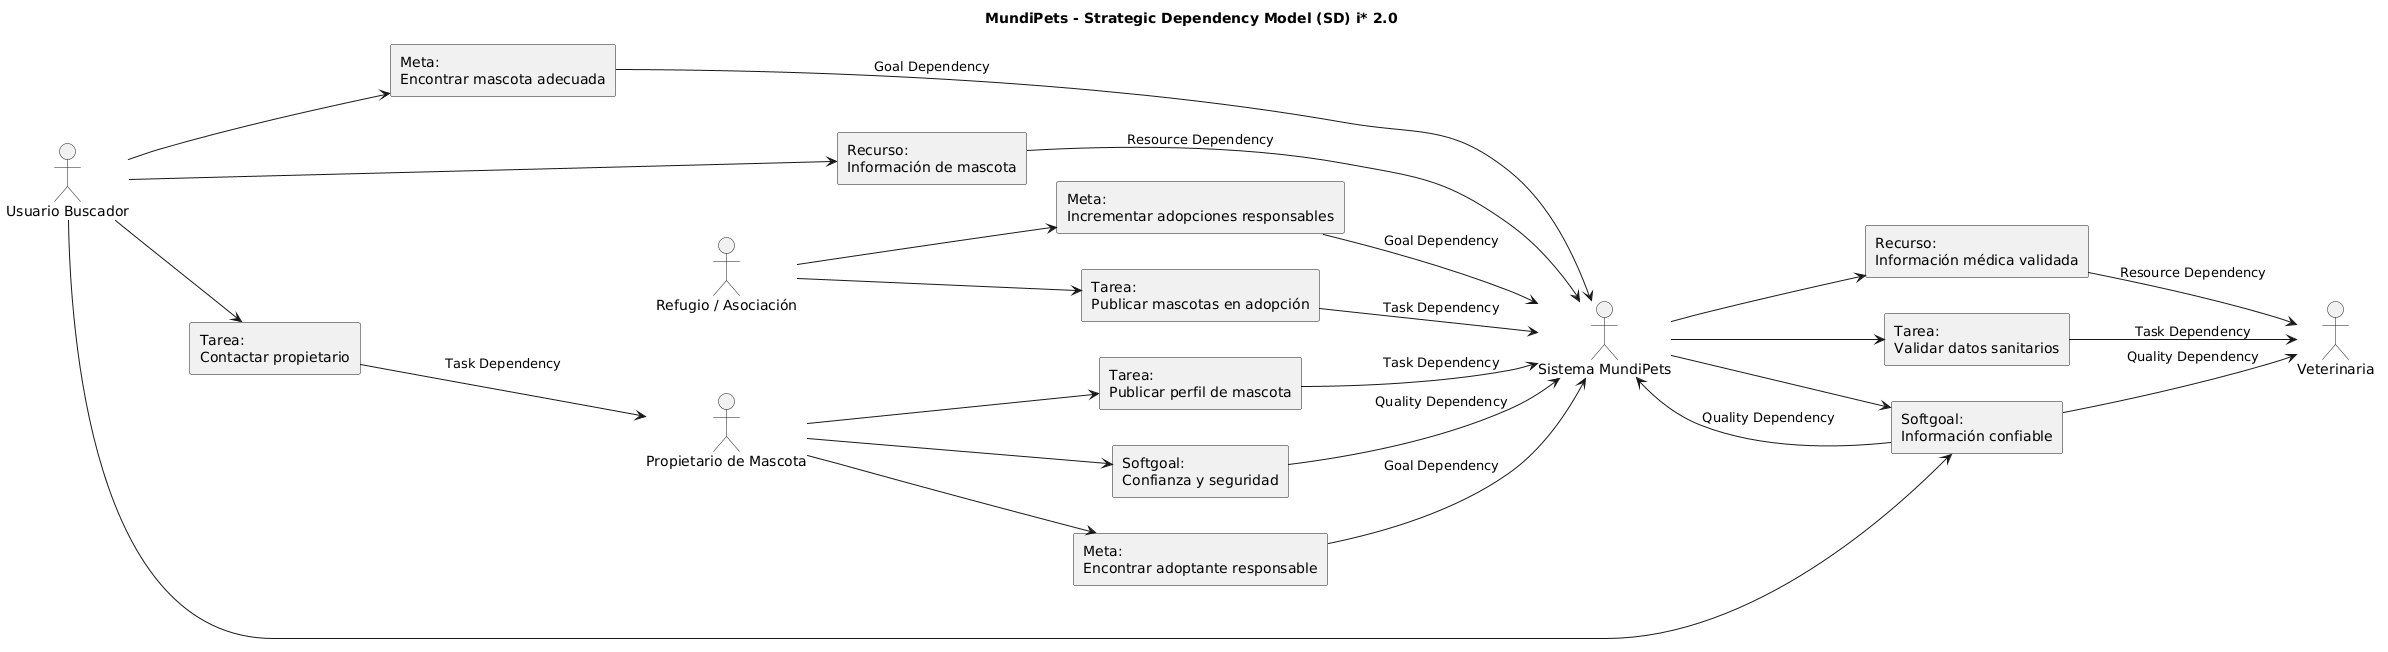
\includegraphics[width=\textwidth]{sd_model.png}
  \caption{Strategic Dependency Model (SD) del sistema MundiPets.}
  \label{fig:sd_model}
\end{figure}

\begin{table}[H]
\caption{Dependencias del SD Model}
\label{tab:sd_dependencias}
\begin{tabularx}{\textwidth}{|l|l|l|X|}
\hline
\textbf{Depender} & \textbf{Dependee} & \textbf{Tipo} & \textbf{Dependum (elemento dependido)} \\
\hline
Propietario de Mascota & Sistema MundiPets & Meta & Encontrar adoptante responsable \\
\hline
Propietario de Mascota & Sistema MundiPets & Tarea & Publicar perfil de mascota \\
\hline
Usuario Buscador & Sistema MundiPets & Meta & Buscar mascota adecuada \\
\hline
Usuario Buscador & Sistema MundiPets & Recurso & Información de mascota \\
\hline
Usuario Buscador & Propietario de Mascota & Tarea & Contactar propietario \\
\hline
Sistema MundiPets & Veterinaria & Recurso & Información médica validada \\
\hline
Sistema MundiPets & Veterinaria & Tarea & Validar datos sanitarios \\
\hline
Refugio o Asociación & Sistema MundiPets & Tarea & Publicar mascotas en adopción \\
\hline
Refugio o Asociación & Sistema MundiPets & Meta & Incrementar adopciones responsables \\
\hline
Propietario de Mascota & Sistema MundiPets & Meta blanda & Confianza y seguridad \\
\hline
Usuario Buscador & Sistema MundiPets & Meta blanda & Información confiable \\
\hline
Sistema MundiPets & Veterinaria & Meta blanda & Información confiable \\
\hline
\end{tabularx}
\end{table}

\subsection{Strategic Rationale Model (SR) del Actor Principal}

El modelo SR del actor principal, Sistema MundiPets, representa el
razonamiento interno necesario para cumplir la meta general de gestionar
adopciones y cruces responsables de mascotas. Para lograr esta meta, el
sistema debe gestionar perfiles de mascotas, facilitar la búsqueda,
permitir la comunicación entre usuarios y administrar información médica
relevante. Estas tareas se relacionan con recursos como datos de mascota,
historial médico, catálogo de mascotas y datos de contacto.

Además, el modelo considera metas blandas como seguridad, confiabilidad,
usabilidad y bienestar animal. La validación de información médica
contribuye positivamente (\textit{MAKE}/\textit{HELP}) a la confiabilidad
del sistema, mientras que la publicación de mascotas sin información
verificada podría afectar negativamente la seguridad y el bienestar
animal. Por ello, el SR permite observar cómo las funcionalidades internas
del sistema apoyan o perjudican los objetivos de calidad esperados.

\begin{figure}[H]
  \centering
  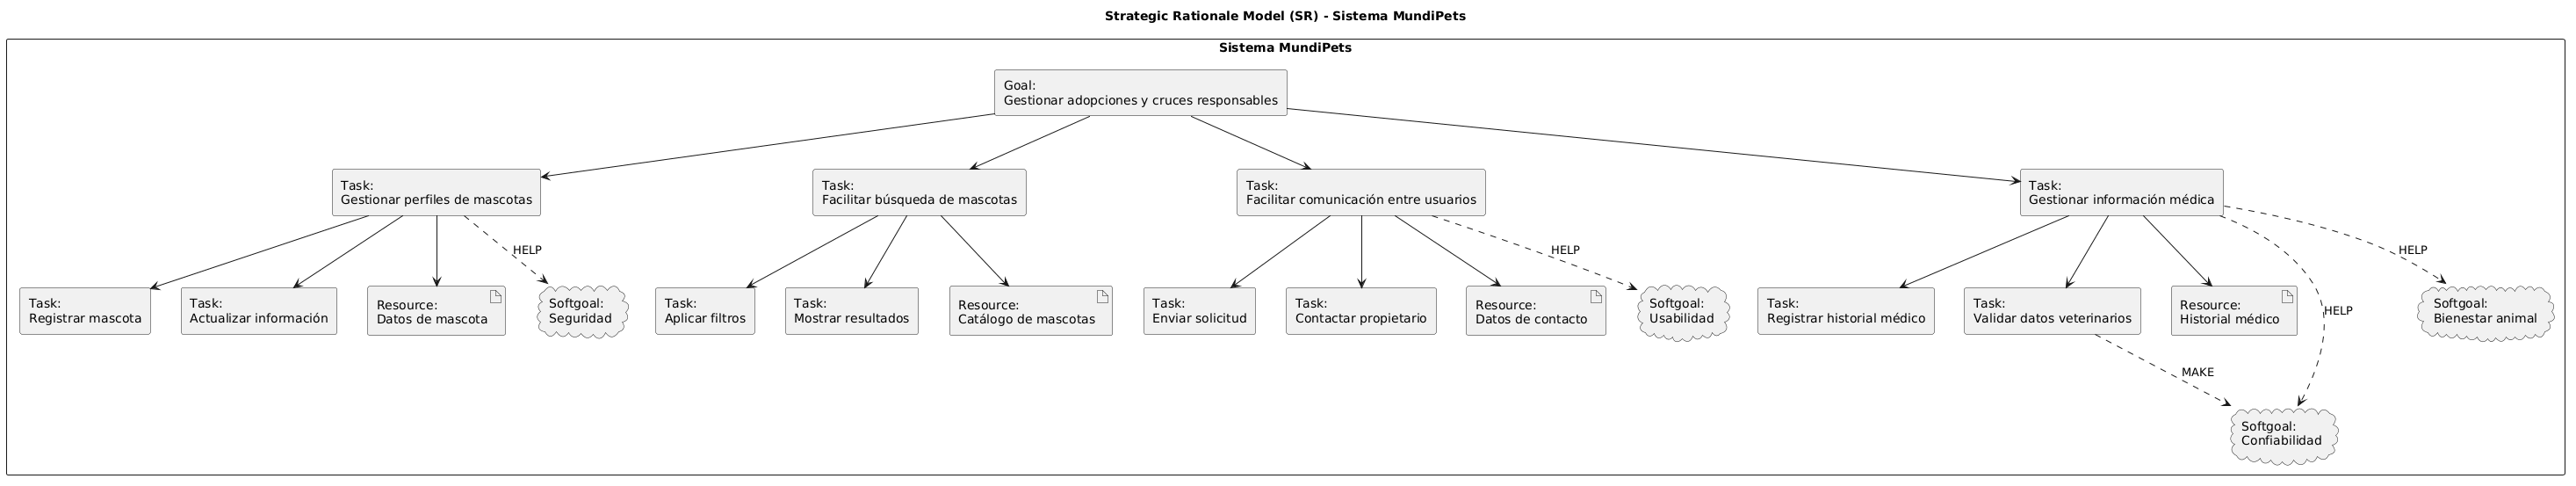
\includegraphics[width=\textwidth]{sr_model.png}
  \caption{Strategic Rationale Model (SR) del actor principal: Sistema
  MundiPets.}
  \label{fig:sr_model}
\end{figure}

\subsection{Especificación Textual de Metas Principales}

\begin{table}[H]
\caption{Especificación textual de metas principales}
\label{tab:metas}
\begin{tabularx}{\textwidth}{|l|X|l|}
\hline
\textbf{Meta} & \textbf{Especificación textual (7 reglas, Pohl~\cite{pohl2025})} & \textbf{NFR asociado} \\
\hline
M-01 -- Gestionar perfiles de mascotas &
El sistema MundiPets deberá permitir que los propietarios registren
perfiles de sus mascotas con información básica, médica y de
comportamiento (RF-01), de forma que otros usuarios puedan conocer datos
relevantes antes de iniciar un proceso de adopción o cruza. Actor
principal: Propietario de mascota. Tipo: \textit{hard goal}. Resultado
esperado: perfil de mascota creado y visible en la plataforma. &
RNF-01 \\
\hline
M-02 -- Facilitar la búsqueda de mascotas &
El sistema deberá permitir que los usuarios buscadores encuentren mascotas
disponibles mediante criterios como especie, raza, edad, estado de salud,
ubicación y finalidad del proceso (RF-03, RF-04), de modo que la búsqueda
sea rápida y organizada. Actor principal: Usuario buscador. Tipo:
\textit{hard goal}. Resultado esperado: lista de mascotas filtrada según
las preferencias del usuario. &
RNF-05 \\
\hline
M-03 -- Facilitar la comunicación entre usuarios &
El sistema deberá permitir la comunicación entre propietarios, adoptantes
interesados y usuarios que buscan cruza (RF-05, RF-06, RF-08, RF-09), de
forma que se puedan coordinar acuerdos, resolver dudas y continuar el
proceso dentro de la plataforma. Actor principal: Propietario / Usuario
buscador. Tipo: \textit{hard goal}. Resultado esperado: solicitud o mensaje
enviado correctamente. &
RNF-02 \\
\hline
M-04 -- Validar información médica de mascotas &
El sistema deberá permitir registrar y consultar información médica
relevante, como vacunas, desparasitaciones, enfermedades previas y
controles veterinarios (RF-07), de forma que los procesos de adopción y
cruza sean más confiables. Actor principal: Veterinaria / Sistema
MundiPets. Tipo: \textit{hard goal}. Resultado esperado: información médica
registrada o validada. &
RNF-SEG-01 \\
\hline
M-05 -- Garantizar confianza y seguridad en los procesos &
El sistema deberá proteger la información sensible de usuarios y mascotas,
además de promover procesos responsables de adopción y cruza. Esta meta se
considera \textit{softgoal}, ya que su cumplimiento depende de la
percepción de confianza, seguridad y transparencia de los usuarios. Actor
principal: Sistema MundiPets. Resultado esperado: mayor percepción de
seguridad y confianza en la plataforma. &
RNF-01, RNF-07 \\
\hline
\end{tabularx}
\end{table}

\textbf{Lectura interpretativa del modelo:}

El modelo de dependencias estratégicas (SD) evidencia que el Sistema
MundiPets actúa como el actor central de la solución, ya que concentra las
principales dependencias de los stakeholders identificados. Los
propietarios de mascotas dependen del sistema para publicar perfiles y
encontrar adoptantes responsables, mientras que los usuarios buscadores
dependen de la plataforma para localizar mascotas adecuadas y acceder a
información confiable. Asimismo, los refugios y asociaciones protectoras
utilizan el sistema para incrementar las oportunidades de adopción,
ampliando la visibilidad de los animales bajo su cuidado, mientras que la
veterinaria proporciona recursos y validaciones médicas que fortalecen la
confiabilidad de la información registrada.

El actor con mayor poder de bloqueo es la Veterinaria: si la
dependencia de tipo recurso ``Información médica validada'' (Sistema
MundiPets~$\rightarrow$~Veterinaria) no se satisface --por ejemplo, si no
hay veterinarias disponibles para validar perfiles-- entonces el requisito
RF-07 y su requisito de seguridad derivado RNF-SEG-01 no podrían cumplirse,
lo que degradaría la meta blanda de confiabilidad (M-05) para todos los
demás actores. De forma similar, si el Sistema MundiPets no satisface la
dependencia de recurso ``Información de mascota'' hacia el Usuario
Buscador, el requisito RF-03 (búsqueda) quedaría sin contenido útil,
afectando directamente la meta M-02. El análisis muestra que la calidad de
la información y la seguridad de los procesos constituyen factores críticos
para el éxito de la plataforma, ya que influyen directamente en la
confianza de los usuarios y en el bienestar de las mascotas involucradas.

\newpage

% ============================================================
%  SECCIÓN 7 -- CASOS DE USO Y USER STORIES (PASO 5)
% ============================================================
\section{Modelado de Escenarios: Casos de Uso y User Stories (Paso 5)}

\subsection{Diagrama de Casos de Uso}

\begin{figure}[H]
  \centering
  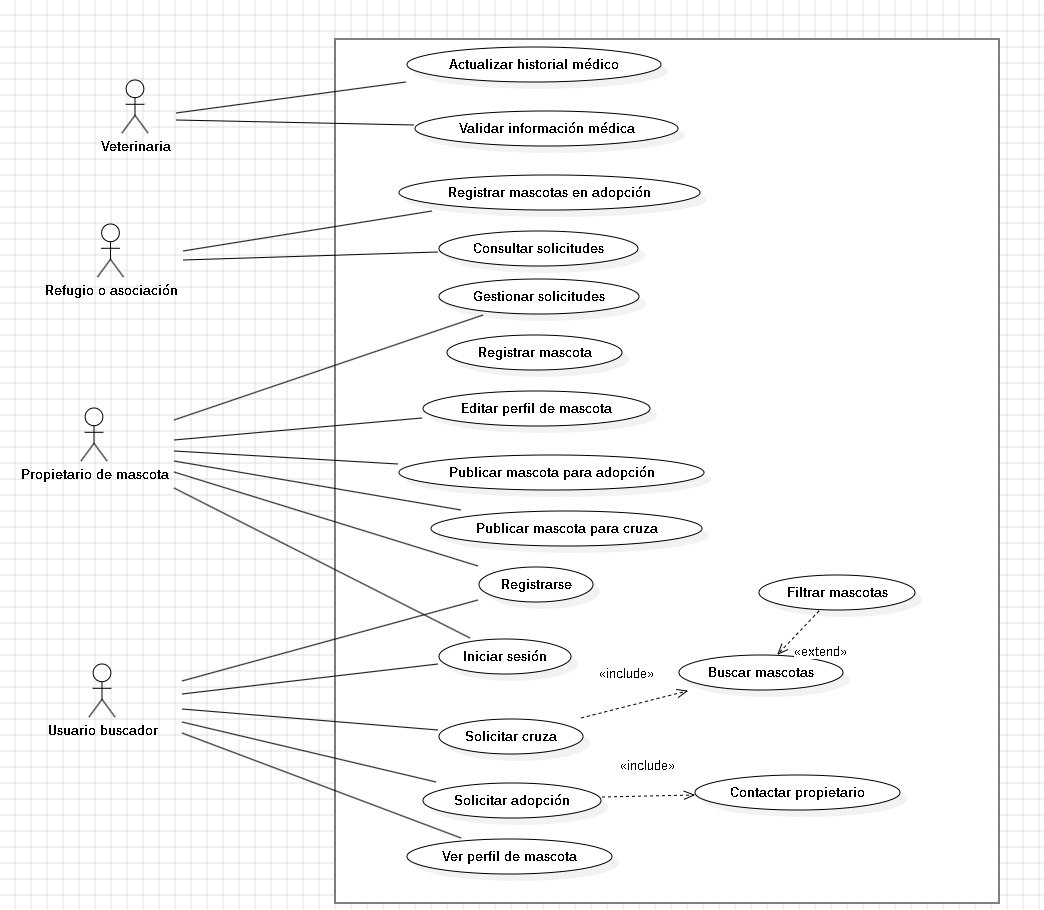
\includegraphics[width=\textwidth]{diagrama_cu.png}
  \caption{Diagrama de casos de uso del sistema MundiPets.}
  \label{fig:diagrama_cu}
\end{figure}

\subsection{Especificaciones Textuales de Tres Casos de Uso}

% ── CU-01 ───────────────────────────────────────────────────
\subsubsection{CU-01: Registrar Mascota}

\begin{table}[H]
\caption{Especificación textual de CU-01}
\label{tab:cu01}
\begin{tabularx}{\textwidth}{|l|X|}
\hline
\textbf{Identificador}       & CU-01 \\
\hline
\textbf{Nombre}              & Registrar mascota \\
\hline
\textbf{Actores}             & Primario: Propietario de mascota. Secundario: Sistema MundiPets \\
\hline
\textbf{Precondiciones}      & \begin{enumerate}[leftmargin=*,topsep=0pt]
                                 \item El propietario debe estar registrado e iniciar sesión en la plataforma.
                               \end{enumerate} \\
\hline
\textbf{Flujo principal}     & \begin{enumerate}[leftmargin=*,topsep=0pt]
                                 \item El propietario accede a la opción ``Registrar mascota''.
                                 \item El sistema muestra el formulario de registro.
                                 \item El propietario ingresa nombre, especie, raza, edad, sexo, estado reproductivo, vacunas, desparasitaciones y comportamiento.
                                 \item El propietario adjunta fotografías de la mascota.
                                 \item El sistema valida que los campos obligatorios estén completos.
                                 \item El propietario confirma el registro.
                                 \item El sistema guarda la información y muestra un mensaje de registro exitoso.
                               \end{enumerate} \\
\hline
\textbf{Flujos alternativos} & \textbf{FA-1} (bifurca en paso~5): si faltan datos obligatorios, el sistema muestra un mensaje indicando los campos pendientes y no permite guardar hasta completarlos. \\
\hline
\textbf{Excepciones}         & \textbf{E-1} (bifurca en paso~7): si ocurre un error de conexión, el sistema informa al usuario que no se pudo registrar la mascota y solicita intentar nuevamente. \\
\hline
\textbf{Postcondiciones}     & \begin{enumerate}[leftmargin=*,topsep=0pt]
                                 \item La mascota queda registrada y disponible en el perfil del propietario.
                               \end{enumerate} \\
\hline
\textbf{Requisitos asociados} & RF-01, RF-02, RNF-01 \\
\hline
\end{tabularx}
\end{table}

% ── CU-02 ───────────────────────────────────────────────────
\subsubsection{CU-02: Buscar Mascota}

\begin{table}[H]
\caption{Especificación textual de CU-02}
\label{tab:cu02}
\begin{tabularx}{\textwidth}{|l|X|}
\hline
\textbf{Identificador}       & CU-02 \\
\hline
\textbf{Nombre}              & Buscar mascota \\
\hline
\textbf{Actores}             & Primario: Usuario buscador. Secundario: Sistema MundiPets \\
\hline
\textbf{Precondiciones}      & \begin{enumerate}[leftmargin=*,topsep=0pt]
                                 \item El usuario debe haber ingresado a la plataforma.
                               \end{enumerate} \\
\hline
\textbf{Flujo principal}     & \begin{enumerate}[leftmargin=*,topsep=0pt]
                                 \item El usuario accede a la sección ``Buscar mascotas''.
                                 \item El sistema muestra el catálogo de mascotas disponibles (vista resumida, según acuerdo de la Sección~\ref{sec:conflictos}).
                                 \item El usuario aplica filtros como especie, raza, edad, ubicación, estado de salud y finalidad.
                                 \item El sistema procesa los criterios seleccionados.
                                 \item El sistema muestra los resultados coincidentes, incluyendo el estado de verificación veterinaria.
                                 \item El usuario selecciona una mascota para revisar su perfil.
                               \end{enumerate} \\
\hline
\textbf{Flujos alternativos} & \textbf{FA-1} (bifurca en paso~5): si no existen mascotas que coincidan con los filtros, el sistema muestra el mensaje ``No se encontraron resultados'' y permite modificar los criterios de búsqueda. \\
\hline
\textbf{Excepciones}         & \textbf{E-1} (bifurca en paso~2): si ocurre un error al cargar el catálogo, el sistema informa el problema y permite reintentar la búsqueda. \\
\hline
\textbf{Postcondiciones}     & \begin{enumerate}[leftmargin=*,topsep=0pt]
                                 \item El sistema muestra una lista de mascotas que coinciden con los filtros seleccionados.
                               \end{enumerate} \\
\hline
\textbf{Requisitos asociados} & RF-03, RF-04, RNF-05 \\
\hline
\end{tabularx}
\end{table}

% ── CU-03 ───────────────────────────────────────────────────
\subsubsection{CU-03: Solicitar Adopción}

\begin{table}[H]
\caption{Especificación textual de CU-03}
\label{tab:cu03}
\begin{tabularx}{\textwidth}{|l|X|}
\hline
\textbf{Identificador}       & CU-03 \\
\hline
\textbf{Nombre}              & Solicitar adopción \\
\hline
\textbf{Actores}             & Primario: Usuario buscador. Secundario: Propietario de mascota, Sistema MundiPets \\
\hline
\textbf{Precondiciones}      & \begin{enumerate}[leftmargin=*,topsep=0pt]
                                 \item El usuario debe haber iniciado sesión y seleccionado una mascota disponible para adopción.
                               \end{enumerate} \\
\hline
\textbf{Flujo principal}     & \begin{enumerate}[leftmargin=*,topsep=0pt]
                                 \item El usuario consulta el perfil completo de una mascota.
                                 \item El usuario selecciona la opción ``Solicitar adopción''.
                                 \item El sistema muestra un formulario de solicitud.
                                 \item El usuario ingresa la información requerida (entorno, condiciones de vivienda, disponibilidad).
                                 \item El sistema valida los datos ingresados.
                                 \item El usuario confirma el envío de la solicitud.
                                 \item El sistema registra la solicitud y notifica al propietario.
                                 \item El propietario puede revisar la solicitud desde su cuenta (CU asociado: Consultar solicitudes).
                               \end{enumerate} \\
\hline
\textbf{Flujos alternativos} & \textbf{FA-1} (bifurca en paso~6): si el usuario cancela la operación antes de confirmar, la solicitud no se registra y el sistema regresa al perfil de la mascota. \\
\hline
\textbf{Excepciones}         & \textbf{E-1} (bifurca en paso~2): si la mascota ya no se encuentra disponible para adopción, el sistema informa al usuario y bloquea el envío de nuevas solicitudes. \\
\hline
\textbf{Postcondiciones}     & \begin{enumerate}[leftmargin=*,topsep=0pt]
                                 \item La solicitud de adopción queda registrada y es enviada al propietario de la mascota.
                               \end{enumerate} \\
\hline
\textbf{Requisitos asociados} & RF-05, RF-06, RNF-01 \\
\hline
\end{tabularx}
\end{table}

\subsection{Cinco User Stories con Criterios de Aceptación BDD}

% ── US-01 ───────────────────────────────────────────────────
\subsubsection{US-01}

\begin{mdframed}[style=guia]
\textit{US-01. Como} propietario de mascota, \textit{quiero} registrar el
perfil de mi mascota \textit{para} publicarla en procesos de adopción o
cruza.
\end{mdframed}

\textbf{INVEST:} Independiente: Sí \quad Negociable: Sí \quad
Valiosa: Sí \quad Estimable: Sí \quad
Pequeña: Sí \quad Testeable: Sí

\textit{La historia es independiente porque puede implementarse sin
depender de otras funcionalidades de búsqueda o adopción; es valiosa
porque sin el registro del perfil no existe contenido en la plataforma; es
estimable y pequeña porque corresponde a un único formulario, y es
testeable porque puede verificarse con datos de entrada concretos.}

\textbf{Criterios de aceptación:}
\begin{enumerate}[leftmargin=*]
  \item \textit{Dado} que el propietario ha iniciado sesión en MundiPets,
  \textit{cuando} ingresa los datos obligatorios de la mascota y confirma el
  registro, \textit{entonces} el sistema guarda el perfil de la mascota y
  muestra un mensaje de registro exitoso.
  \item \textit{Dado} que el propietario adjunta fotografías de la mascota,
  \textit{cuando} el formulario se envía con al menos una fotografía válida,
  \textit{entonces} el sistema asocia las imágenes al perfil de la mascota.
  \item \textit{Dado} que el propietario intenta registrar una mascota,
  \textit{cuando} deja campos obligatorios vacíos, \textit{entonces} el
  sistema muestra una alerta indicando los datos faltantes y no guarda el
  perfil.
\end{enumerate}
\textbf{CU asociado:} CU-01 \quad \textbf{Requisito:} RF-01

% ── US-02 ───────────────────────────────────────────────────
\subsubsection{US-02}

\begin{mdframed}[style=guia]
\textit{US-02. Como} usuario buscador, \textit{quiero} filtrar mascotas
disponibles \textit{para} encontrar una mascota que se ajuste a mis
preferencias.
\end{mdframed}

\textbf{INVEST:} Independiente: Sí \quad Negociable: Sí \quad
Valiosa: Sí \quad Estimable: Sí \quad
Pequeña: Sí \quad Testeable: Sí

\textit{La historia es negociable porque los criterios de filtro pueden
ajustarse según la disponibilidad de datos; es valiosa porque reduce el
tiempo de búsqueda del usuario (RNF-05); es pequeña porque se limita a la
lógica de filtrado sobre un catálogo ya existente, y es testeable mediante
combinaciones de filtros con resultados conocidos.}

\textbf{Criterios de aceptación:}
\begin{enumerate}[leftmargin=*]
  \item \textit{Dado} que el usuario está en la sección de búsqueda,
  \textit{cuando} selecciona filtros como especie, raza, edad o ubicación,
  \textit{entonces} el sistema muestra las mascotas que coinciden con los
  criterios seleccionados en un tiempo $\leq$ 3 segundos.
  \item \textit{Dado} que el usuario aplica un filtro de compatibilidad para
  cruza, \textit{cuando} el sistema procesa la consulta, \textit{entonces}
  muestra únicamente mascotas con perfil médico validado y compatible.
  \item \textit{Dado} que no existen mascotas que coincidan con los
  filtros, \textit{cuando} el usuario realiza la búsqueda, \textit{entonces}
  el sistema muestra un mensaje indicando que no se encontraron resultados.
\end{enumerate}
\textbf{CU asociado:} CU-02 \quad \textbf{Requisito:} RF-03, RF-04

% ── US-03 ───────────────────────────────────────────────────
\subsubsection{US-03}

\begin{mdframed}[style=guia]
\textit{US-03. Como} usuario buscador, \textit{quiero} solicitar la
adopción de una mascota \textit{para} iniciar el proceso con el propietario
o refugio responsable.
\end{mdframed}

\textbf{INVEST:} Independiente: Sí \quad Negociable: Sí \quad
Valiosa: Sí \quad Estimable: Sí \quad
Pequeña: Sí \quad Testeable: Sí

\textit{La historia es valiosa porque representa el punto de conversión
principal de la plataforma; es estimable porque depende de un formulario y
una notificación; es pequeña porque no incluye el flujo completo de
seguimiento post-adopción (cubierto por US-05), y es testeable verificando
el estado de la solicitud tras su envío.}

\textbf{Criterios de aceptación:}
\begin{enumerate}[leftmargin=*]
  \item \textit{Dado} que el usuario ha iniciado sesión, \textit{cuando}
  selecciona una mascota disponible y envía la solicitud de adopción,
  \textit{entonces} el sistema registra la solicitud y notifica al
  propietario o refugio.
  \item \textit{Dado} que el usuario completa el formulario de solicitud,
  \textit{cuando} indica información sobre el entorno y condiciones de
  vivienda, \textit{entonces} el sistema incluye esa información en la
  solicitud para que el propietario la revise (RF-08).
  \item \textit{Dado} que una mascota ya no está disponible, \textit{cuando}
  el usuario intenta solicitar su adopción, \textit{entonces} el sistema
  bloquea la solicitud e informa que la mascota no está disponible.
\end{enumerate}
\textbf{CU asociado:} CU-03 \quad \textbf{Requisito:} RF-05, RF-06

% ── US-04 ───────────────────────────────────────────────────
\subsubsection{US-04}

\begin{mdframed}[style=guia]
\textit{US-04. Como} veterinaria, \textit{quiero} validar la información
médica de una mascota \textit{para} aumentar la confianza en los procesos
de adopción o cruza.
\end{mdframed}

\textbf{INVEST:} Independiente: Sí \quad Negociable: Sí \quad
Valiosa: Sí \quad Estimable: Sí \quad
Pequeña: Sí \quad Testeable: Sí

\textit{La historia es valiosa porque sustenta la meta blanda de
confiabilidad (M-05) y el requisito de seguridad RNF-SEG-01; es estimable y
pequeña porque corresponde a una acción de revisión y marcado de estado, y
es testeable verificando el cambio de estado del perfil tras la
validación.}

\textbf{Criterios de aceptación:}
\begin{enumerate}[leftmargin=*]
  \item \textit{Dado} que la veterinaria accede al historial médico de una
  mascota, \textit{cuando} verifica vacunas, desparasitaciones y controles,
  \textit{entonces} el sistema marca la información médica como validada en
  un tiempo $\leq$ 5 segundos (RNF-SEG-01).
  \item \textit{Dado} que un perfil ha sido validado, \textit{cuando} un
  usuario buscador consulta el catálogo, \textit{entonces} el sistema
  muestra una insignia de ``información verificada'' en dicho perfil.
  \item \textit{Dado} que la veterinaria detecta información incompleta o
  inconsistente, \textit{cuando} intenta validar el perfil, \textit{entonces}
  el sistema le permite registrar observaciones y no marca el perfil como
  validado.
\end{enumerate}
\textbf{CU asociado:} Validar información médica \quad \textbf{Requisito:} RF-07, RNF-SEG-01

% ── US-05 ───────────────────────────────────────────────────
\subsubsection{US-05}

\begin{mdframed}[style=guia]
\textit{US-05. Como} propietario de mascota, \textit{quiero} consultar las
solicitudes recibidas \textit{para} evaluar interesados en adopción o
cruza.
\end{mdframed}

\textbf{INVEST:} Independiente: Sí \quad Negociable: Sí \quad
Valiosa: Sí \quad Estimable: Sí \quad
Pequeña: Sí \quad Testeable: Sí

\textit{La historia es valiosa porque cierra el ciclo iniciado en US-03; es
negociable en cuanto al orden o formato de presentación de las solicitudes;
es pequeña porque corresponde a una vista de consulta y a una acción de
respuesta (aceptar/rechazar), y es testeable verificando el listado de
solicitudes y el cambio de estado tras la decisión del propietario.}

\textbf{Criterios de aceptación:}
\begin{enumerate}[leftmargin=*]
  \item \textit{Dado} que el propietario tiene mascotas publicadas,
  \textit{cuando} ingresa a la sección de solicitudes, \textit{entonces} el
  sistema muestra las solicitudes recibidas con la información del
  interesado (RF-08).
  \item \textit{Dado} que el propietario revisa una solicitud, \textit{cuando}
  decide aceptarla, \textit{entonces} el sistema notifica al usuario
  buscador y actualiza el estado de la mascota a ``en proceso de adopción''
  (RF-09).
  \item \textit{Dado} que el propietario revisa una solicitud, \textit{cuando}
  decide rechazarla, \textit{entonces} el sistema notifica al usuario
  buscador con el motivo de rechazo y mantiene la mascota disponible
  (RF-09).
\end{enumerate}
\textbf{CU asociado:} Consultar solicitudes \quad \textbf{Requisito:} RF-08, RF-09

\subsection{Misuse Scenario (Requisito de Seguridad)}

\begin{table}[H]
\caption{Misuse scenario para requisito de seguridad}
\label{tab:misuse}
\begin{tabularx}{\textwidth}{|l|X|}
\hline
\textbf{Identificador}      & MS-01 \\
\hline
\textbf{Nombre}             & Publicación de información falsa sobre una mascota \\
\hline
\textbf{Actor malicioso}    & Usuario no confiable, registrado en la plataforma sin verificación previa, motivado por obtener una adopción o cruza sin pasar por controles veterinarios. \\
\hline
\textbf{Objetivo del ataque} & Registrar o publicar información falsa sobre una mascota para lograr adopciones o cruces sin controles adecuados. \\
\hline
\textbf{Secuencia del abuso} & \begin{enumerate}[leftmargin=*,topsep=0pt]
                                 \item El usuario crea una cuenta en MundiPets.
                                 \item Registra una mascota con datos incompletos o falsos.
                                 \item Publica la mascota para adopción o cruza.
                                 \item Otros usuarios visualizan la información como si fuera confiable.
                                 \item Se inicia un proceso de adopción o cruza basado en información incorrecta.
                               \end{enumerate} \\
\hline
\textbf{Daño potencial}      & Adopciones irresponsables, cruces inseguros, pérdida de confianza en la plataforma y afectación al bienestar de las mascotas. \\
\hline
\textbf{Medida de mitigación} & El sistema deberá permitir la validación de información médica por parte de veterinarias y mostrar el estado de verificación del perfil (RF-07). \\
\hline
\textbf{Requisito derivado}  & RNF-SEG-01 -- El sistema deberá marcar claramente los perfiles de mascotas cuya información médica haya sido validada por una veterinaria, diferenciándolos de los perfiles no verificados, en un tiempo de actualización del estado de verificación $\leq$ 5 segundos. \\
\hline
\textbf{Casos de uso relacionados} & CU-01 Registrar mascota, CU-03 Solicitar adopción, Validar información médica \\
\hline
\end{tabularx}
\end{table}

\subsection{Matriz de Trazabilidad}

\begin{longtable}{|c|p{7cm}|c|c|}
	\caption{Matriz de trazabilidad: meta $\rightarrow$ requisito $\rightarrow$ caso de uso $\rightarrow$ user story}
	\label{tab:trazabilidad}\\
	
	\hline
	\textbf{Meta} & \textbf{Requisito} & \textbf{Caso de Uso} & \textbf{User Story} \\
	\hline
	\endfirsthead
	
	\hline
	\textbf{Meta} & \textbf{Requisito} & \textbf{Caso de Uso} & \textbf{User Story} \\
	\hline
	\endhead
	
	M-01 & RF-01 -- Registrar perfil de mascota & UC3 & US-01 \\
	\hline
	
	M-01 & RF-02 -- Actualizar información de mascota & UC4 & US-01 \\
	\hline
	
	M-02 & RF-03 -- Buscar mascotas & UC7 & US-02 \\
	\hline
	
	M-02 & RF-04 -- Filtrar mascotas / compatibilidad & UC8 & US-02 \\
	\hline
	
	M-03 & RF-05 -- Solicitar adopción/cruza & UC10, UC11 & US-03 \\
	\hline
	
	M-03 & RF-06 -- Contactar propietario & UC12 & US-03 \\
	\hline
	
	M-04 & RF-07 -- Validar historial médico & UC14 & US-04 \\
	\hline
	
	M-05 & RNF-SEG-01 -- Perfil verificado & UC14 & US-04 \\
	\hline
	
	M-03 & RF-08 -- Consultar solicitudes & UC13 & US-05 \\
	\hline
	
	M-03 & RF-09 -- Gestionar solicitudes & UC17 & US-05 \\
	\hline
	
	M-05 & RNF-01 -- Protección de datos médicos sensibles & UC3, UC10, UC11, UC12 & US-01, US-03 \\
	\hline
	
	M-02 & RNF-05 -- Tiempo de respuesta de búsqueda & UC7, UC8 & US-02 \\
	\hline
	
\end{longtable}

La matriz de trazabilidad permite verificar la relación existente entre las
metas del sistema, los requisitos identificados durante la elicitación, los
casos de uso definidos y las historias de usuario elaboradas. Esta relación
garantiza que cada funcionalidad propuesta contribuya al cumplimiento de
los objetivos del sistema MundiPets y facilita la validación de requisitos
durante las etapas posteriores del desarrollo. Los requisitos RF-10
(exportación a PDF) y RF-11 (búsqueda de clínicas por proximidad), al ser de
prioridad \textit{Could} (Sección~5.3), no cuentan con caso de uso ni user
story dedicados en esta práctica; quedan documentados como funcionalidades
de una versión posterior del PFC.

\newpage

% ============================================================
%  SECCIÓN 8 -- CONCLUSIONES
% ============================================================
\section{Conclusiones}

La aplicación combinada de la entrevista estructurada y el cuestionario
resultó efectiva para capturar requisitos del sistema MundiPets desde dos
perspectivas complementarias. La entrevista permitió obtener información
profunda y especializada por parte de los médicos veterinarios, en
particular sobre los campos que debe contener el perfil médico de una
mascota y sobre los criterios para evaluar una adopción responsable; sin
esta técnica, difícilmente se habrían identificado requisitos como la
validación veterinaria del historial (RF-07) o la protección de
enfermedades catastróficas (RNF-01). El cuestionario, implementado mediante
Google Forms, permitió recopilar y consolidar las opiniones de los
participantes de manera organizada, aportando una cuantificación de
tendencias (por ejemplo, el 93\,\% de valoraciones altas en los ítems
Likert) que facilitó la priorización objetiva de funcionalidades. La
utilización conjunta de entrevistas y cuestionarios permitió obtener tanto
información cualitativa como cuantitativa, fortaleciendo el proceso de
elicitación y análisis de requisitos, en concordancia con las buenas
prácticas recomendadas por IREB CPRE FL v3.1~\cite{ireb2023}.

El proceso de análisis y clasificación de requisitos, mediante la
aplicación de la metodología MoSCoW y la categorización estricta entre
Requisitos Funcionales (RF) y Requisitos No Funcionales (RNF), permitió una
transición efectiva desde una lista de necesidades crudas hacia un conjunto
priorizado y alineado con los estándares de calidad de software. La
aplicación de la norma ISO/IEC 25010:2023~\cite{iso25010} fue fundamental
para asegurar la adecuación funcional del sistema, permitiendo que la
percepción del equipo evolucionara de una visión basada en deseos
intuitivos a una basada en criterios de impacto real para el usuario final.
La priorización cambió radicalmente nuestra percepción inicial: requisitos
que inicialmente clasificamos como \textit{Could} (deseables), como la
protección de datos médicos sensibles (RNF-01) y el cumplimiento normativo
del modelo de datos (RR-01), fueron recategorizados como \textit{Must}
(obligatorios) tras el análisis de riesgos y la validación con los
stakeholders. Entendimos que el éxito de MundiPets no radica únicamente en
su funcionalidad, sino en la seguridad y confiabilidad de la información
clínica, elementos que anteriormente subestimamos. Esta clasificación
permitió establecer una base técnica sólida, asegurando que el sistema no
solo cumpla con las expectativas del usuario, sino que garantice la calidad
del producto final desde su concepción.

El modelado mediante i* 2.0~\cite{yu2011} reveló que el Sistema MundiPets
concentra la mayor parte de las dependencias estratégicas del ecosistema,
pero que la Veterinaria es el actor con mayor poder de bloqueo: la
dependencia de recurso ``información médica validada'' es la única vía por
la cual el sistema puede satisfacer la meta blanda de confiabilidad (M-05)
y el requisito de seguridad RNF-SEG-01. Si esta dependencia no se
satisface --por ejemplo, por falta de disponibilidad de profesionales
veterinarios dispuestos a validar perfiles-- el requisito RF-07 quedaría
sin cumplir, y con él toda la cadena de confianza que sostiene los procesos
de adopción y cruza modelados en la Sección~7. El modelado realizado
mediante i* 2.0, casos de uso, user stories y el \textit{misuse scenario}
permitió representar de forma organizada las metas, dependencias e
interacciones principales del sistema MundiPets. Estos artefactos ayudaron
a relacionar las necesidades de propietarios, usuarios buscadores, refugios
y veterinarias con funcionalidades concretas del sistema, fortaleciendo la
trazabilidad entre requisitos, escenarios y objetivos del proyecto, en
línea con los principios de modelado orientado a metas descritos por
Pohl~\cite{pohl2025}.

La trazabilidad construida entre las metas, los requisitos consolidados,
los casos de uso y las user stories (Tabla~\ref{tab:trazabilidad}) permitió
verificar que los once requisitos funcionales identificados cuentan con un
origen claro en las metas del sistema, y que las cinco user stories
desarrolladas cubren las metas M-01 a M-05 sin dejar ninguna de ellas sin
cobertura. Este resultado es consistente con las recomendaciones de
ISO/IEC/IEEE 29148~\cite{iso29148} y del SWEBOK v4.0~\cite{swebok2024} sobre
la importancia de mantener trazabilidad bidireccional entre requisitos y
artefactos de diseño, ya que facilita identificar el impacto de un cambio
(por ejemplo, si se modifica RF-07, es posible identificar de inmediato que
afecta a CU ``Validar información médica'', a US-04 y a la meta blanda
M-05). Los dos únicos requisitos que quedaron sin cobertura de caso de uso o
user story dedicados fueron RF-10 (exportación del historial a PDF) y RF-11
(búsqueda de clínicas por proximidad); ambos fueron clasificados como
\textit{Could} en la priorización MoSCoW (Sección~5.3), por lo que su
ausencia de modelado detallado en esta práctica es coherente con su menor
prioridad y se documenta como trabajo pendiente para una iteración
posterior del PFC.

La aplicación de la ingeniería de requisitos en el desarrollo de software
dentro del contexto ecuatoriano representa un factor determinante para el
éxito de proyectos que buscan solucionar problemáticas locales, como la
gestión veterinaria integral. La elicitación y el análisis riguroso
permiten que el software no solo sea una herramienta técnica, sino una
solución adaptada a las necesidades reales, culturales y sociales de
nuestro entorno. Como señala Sommerville~\cite{sommerville2018}, un
análisis de requisitos deficiente es una de las causas principales del
fracaso en el desarrollo de sistemas, ya que conlleva a la entrega de
productos que no resuelven el problema del cliente, incrementando costos de
mantenimiento y retrabajo. El impacto de aplicar correctamente este proceso
es la creación de sistemas robustos, éticos y orientados a la experiencia
del usuario, evitando el desarrollo de soluciones desconectadas de la
realidad del país. Por el contrario, cuando se omite este proceso, los
sistemas tienden a la obsolescencia temprana y al desuso, desperdiciando
recursos y tiempo en funcionalidades irrelevantes. Tal como afirma
Pressman~\cite{pressman2010}, el costo de corregir un error en la etapa de
requisitos es significativamente menor que en fases posteriores, por lo que
la omisión de esta fase compromete la viabilidad económica y técnica del
proyecto. En conclusión, el desarrollo responsable de software en Ecuador
requiere pasar de una visión centrada exclusivamente en la codificación a
una visión fundamentada en la ingeniería de requisitos, garantizando así un
impacto positivo y sostenible en la sociedad.

\newpage

% ============================================================
%  REFERENCIAS
% ============================================================

\printbibliography[heading=bibnumbered, title={Referencias}]

\newpage

% ============================================================
%  SECCIÓN 9 -- ANEXOS
% ============================================================
\section{Anexos}

\subsection{Actas Completas de Entrevistas y Evidencias de Campo}
\label{app:entrevistas}

A continuación se presentan las actas completas de las cinco entrevistas
estructuradas realizadas para la elicitación de requisitos del sistema
MundiPets, seguidas de los formularios de consentimiento informado firmados
por cada participante externo.

\subsubsection{Entrevista \#1}

\begin{table}[H]
\caption{Datos generales de la Entrevista \#1}
\label{tab:datos_e1}
\begin{tabularx}{\textwidth}{|p{4cm}|X|}
\hline
\textbf{Campo} & \textbf{Información} \\
\hline
Fecha & 17/05/2026 \\
\hline
Entrevistado & Chacón Morales Mariella Fernanda \\
\hline
Cargo/Rol & Médico veterinario \\
\hline
Entrevistador & Morales Sánchez Gary Alejandro \\
\hline
Técnica & Entrevista estructurada \\
\hline
\end{tabularx}
\end{table}

\begin{longtable}{|p{7.5cm}|p{7.5cm}|}
\caption{Preguntas y respuestas de la Entrevista \#1}
\label{tab:pr_e1}\\
\hline
\textbf{Pregunta} & \textbf{Respuesta resumida} \\
\hline
\endfirsthead
\hline
\textbf{Pregunta} & \textbf{Respuesta resumida} \\
\hline
\endhead
¿Qué información considera más importante conocer sobre una mascota? & Se considera importante conocer la raza, el temperamento, el entorno, la alimentación, si ha tenido presencia de ectoparásitos, y su plan de vacunación y desparasitación. \\
\hline
¿Qué datos ayudan a entender mejor el estado general de una mascota? & Mediante un examen físico, color y estado del pelaje, coloración de las mucosas, la condición corporal (si están con sobrepeso o debajo del peso normal). \\
\hline
¿Qué antecedentes considera importantes conocer sobre una mascota? & Se considera importante conocer si ha tenido presencia de ectoparásitos. \\
\hline
¿Qué riesgos existen cuando no se conoce suficiente información sobre una mascota? & Se podría enfrentar ante graves problemas de salud, ya que existen riesgos que comprometen la vida del animal, como garrapatas y pulgas. \\
\hline
¿Cómo influye la edad de una mascota en su cuidado y comportamiento? & Cuando son cachorros, aprenden y son traviesos. Cuando alcanzan la madurez sexual, su temperamento se moldea sobre lo aprendido en su etapa de cachorro. \\
\hline
¿Cómo influye la raza en las necesidades de una mascota? & El temperamento influye en la raza, algunas son catalogadas como peligrosas. \\
\hline
¿Qué datos de la mascota considera sensibles? & Enfermedades catastróficas, enfermedades que lo pongan en riesgo de muerte, e intervenciones quirúrgicas. \\
\hline
¿Qué enfermedades o condiciones considera importante registrar en una mascota? & Ectoparásitos, y si ha seguido un plan de vacunación y desparasitación. \\
\hline
¿Qué información involucra el perfil médico de una mascota? & Involucra los datos generales (nombre, raza, etc.), antecedentes (como últimas vacunaciones, presencia de parásitos, enfermedades), condición física, estado reproductivo, cirugías previas y medicina que esté tomando actualmente. \\
\hline
¿Cómo puede verificarse si una mascota cuenta con controles médicos adecuados? & Se recomienda tener un médico veterinario para verificar controles. \\
\hline
¿Cómo evalúa si una adopción puede considerarse responsable? & Saber si el adoptante es responsable, si tiene tiempo y un presupuesto destinado a temas de salud y entretenimiento de la mascota. \\
\hline
¿Qué información considera importante antes de entregar una mascota en adopción? & Antes de entregar una mascota en adopción, se considera importante conocer el entorno donde vivirá el animal y garantizar que exista seguimiento y comunicación durante el proceso de adopción. \\
\hline
¿Cómo afectan las adopciones informales al bienestar animal? & Las adopciones informales pueden afectar negativamente al bienestar animal debido a la falta de seguimiento, poca verificación de los adoptantes y riesgo de abandono. \\
\hline
¿Qué información considera esencial antes de recomendar un cruce entre mascotas? & Antecedentes de enfermedades, como ETS, garrapatas, patologías hereditarias. \\
\hline
¿Cómo puede identificarse si dos mascotas son compatibles entre sí? & La compatibilidad entre dos mascotas puede identificarse considerando factores como la raza, tamaño, edad, temperamento, estado de salud y comportamiento durante la interacción entre ambas. \\
\hline
¿Cómo identifica posibles riesgos en procesos de reproducción entre mascotas? & El médico veterinario identifica los riesgos y transmite a los propietarios cómo prevenirlos. \\
\hline
¿Cómo afectan los cruces irresponsables a las mascotas? & Puede haber personas que usen el cruce para lucrarse. \\
\hline
\end{longtable}

\begin{figure}[H]
  \centering
  
\includegraphics[width=0.85\textwidth]{consentimiento_chacon.png}
  \caption{Formulario de consentimiento informado firmado por la Méd. Vet. Mariella Fernanda Chacón Morales (Entrevista \#1).}
  \label{fig:consentimiento_chacon}
\end{figure}

\subsubsection{Entrevista \#2}

\begin{table}[H]
\caption{Datos generales de la Entrevista \#2}
\label{tab:datos_e2}
\begin{tabularx}{\textwidth}{|p{4cm}|X|}
\hline
\textbf{Campo} & \textbf{Información} \\
\hline
Fecha & 29/05/2026 \\
\hline
Entrevistado & Monserrate Arévalo Bryan Steven \\
\hline
Cargo/Rol & Médico veterinario \\
\hline
Entrevistador & Mendoza Párraga Andy Johel \\
\hline
Técnica & Entrevista estructurada \\
\hline
\end{tabularx}
\end{table}

\begin{longtable}{|p{7.5cm}|p{7.5cm}|}
\caption{Preguntas y respuestas de la Entrevista \#2}
\label{tab:pr_e2}\\
\hline
\textbf{Pregunta} & \textbf{Respuesta resumida} \\
\hline
\endfirsthead
\hline
\textbf{Pregunta} & \textbf{Respuesta resumida} \\
\hline
\endhead
¿Qué información considera más importante conocer sobre una mascota? & La edad, la raza y el control de vacunas y desparasitaciones. \\
\hline
¿Qué datos ayudan a entender mejor el estado general de una mascota? & En consulta es importante saber la alimentación que la mascota lleve, en caso de enfermedad si presenta vómitos o diarrea. \\
\hline
¿Qué antecedentes considera importantes conocer sobre una mascota? & Si ha tenido reacciones alérgicas, si la mascota ha sido esterilizada o no, y si ha sido automedicado. \\
\hline
¿Qué riesgos existen cuando no se conoce suficiente información sobre una mascota? & En las cirugías existen riesgos tanto en la cicatrización de heridas, o de mascotas con problemas cardíacos o respiratorios, que pueden llegar a morir en plena cirugía o en el postoperatorio, por ello es importante realizar exámenes antes. \\
\hline
¿Cómo influye la edad de una mascota en su cuidado y comportamiento? & Si es una mascota salvaje o es muy arisca, al momento de una intervención no va a tener los cuidados necesarios, si es una mascota dócil va a ser más manipulable, y esto ocurre mucho más cuando son adultos. \\
\hline
¿Cómo influye la raza en las necesidades de una mascota? & La raza influye, más que todo cuando son braquiocefálicos, es decir, las mascotas con nariz chata, ya que pueden tener problemas respiratorios, y la predisposición de pacientes con displasia de cadera como lo es el pastor alemán. \\
\hline
¿Qué datos de la mascota considera sensibles? & Sobre todo, la edad. \\
\hline
¿Qué enfermedades o condiciones considera importante registrar en una mascota? & Enfermedades como moquillo o parvo, porque las mascotas que han sufrido de eso, van a presentar secuelas, como diarreas y problemas nerviosos. \\
\hline
¿Qué información involucra el perfil médico de una mascota? & Sobre todo, si ha sido automedicado, datos personales como el nombre, raza, edad, vacunas, signos vitales, temperatura y peso al entrar a la veterinaria. \\
\hline
¿Cómo puede verificarse si una mascota cuenta con controles médicos adecuados? & Con el carnet de vacunación, y si no lo tiene, se puede sacar de algún registro de alguna plataforma virtual ya que hoy en día se utilizan mucho. \\
\hline
¿Cómo evalúa si una adopción puede considerarse responsable? & Nos fijamos en que la persona cuente con un sueldo más o menos estable y que tenga domicilio propio. \\
\hline
¿Qué información considera importante antes de entregar una mascota en adopción? & Que la casa tenga cerramiento y que la vivienda sea propia. \\
\hline
¿Cómo afectan las adopciones informales al bienestar animal? & En la veterinaria sobre todo se dan en adopción mascotas con alguna discapacidad, en caso de ser informal, afectaría mucho no saber con qué otros animales van a convivir. \\
\hline
¿Qué información considera esencial antes de recomendar un cruce entre mascotas? & La raza y el pedigree (genealogía), y que no exista parentesco, es decir que vengan de la misma mamá. \\
\hline
¿Cómo puede identificarse si dos mascotas son compatibles entre sí? & Por la raza. \\
\hline
¿Cómo identifica posibles riesgos en procesos de reproducción entre mascotas? & Existen riesgos cuando son braquiocefálicos, por los problemas respiratorios o cardíacos. \\
\hline
¿Cómo afectan los cruces irresponsables a las mascotas? & Afectan, pueden llegar a presentar deformidad, polidactilia, ciclopía o el síndrome de la foca, que es cuando no tienen las articulaciones bien formadas por el parentesco. \\
\hline
\end{longtable}

\begin{figure}[H]
  \centering
  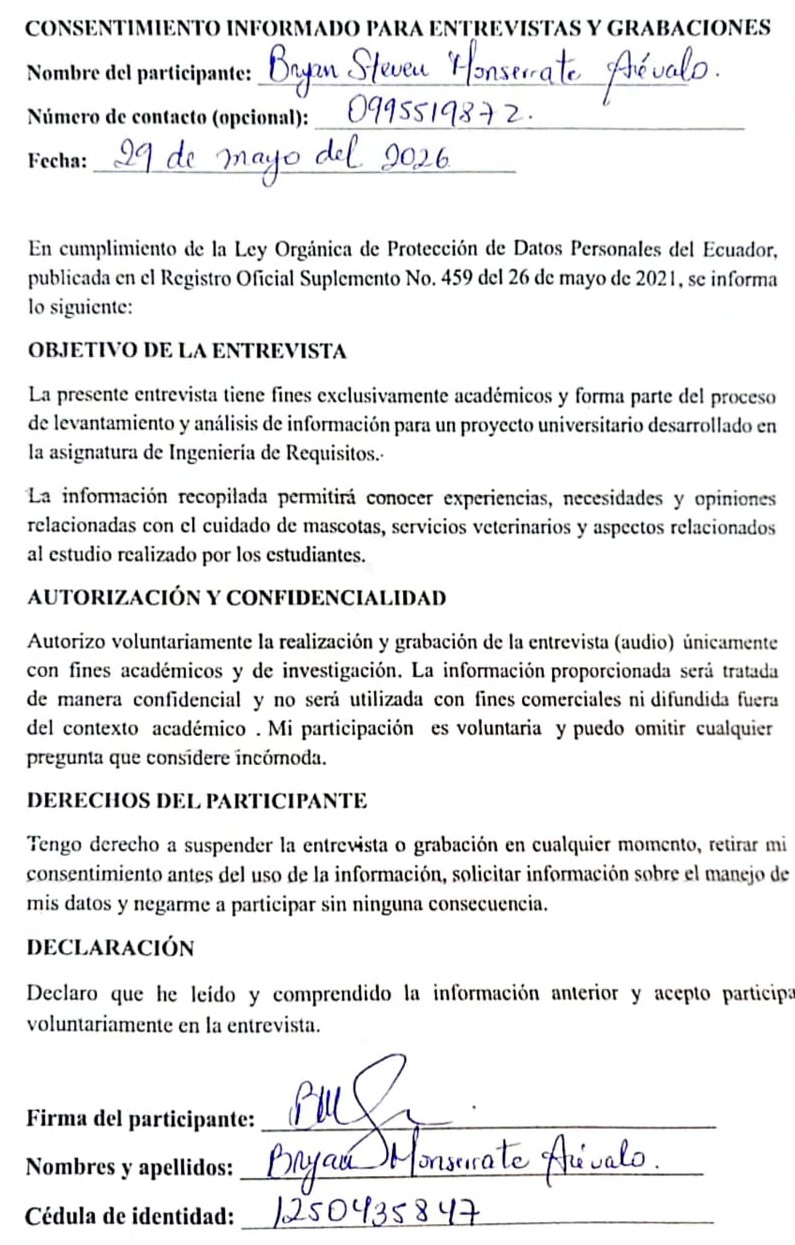
\includegraphics[width=0.85\textwidth]{consentimiento_monserrate.jpeg}
  \caption{Formulario de consentimiento informado firmado por el Méd. Vet. Bryan Steven Monserrate Arévalo (Entrevista \#2).}
  \label{fig:consentimiento_monserrate}
\end{figure}

\subsubsection{Entrevista \#3}

\begin{table}[H]
\caption{Datos generales de la Entrevista \#3}
\label{tab:datos_e3}
\begin{tabularx}{\textwidth}{|p{4cm}|X|}
\hline
\textbf{Campo} & \textbf{Información} \\
\hline
Fecha & 17/05/2026 \\
\hline
Entrevistado & Rosado Palma Kevin Andrés \\
\hline
Cargo/Rol & Veterinario \\
\hline
Entrevistador & Fuertes Arraes Edson Daniel \\
\hline
Técnica & Entrevista estructurada \\
\hline
\end{tabularx}
\end{table}

\begin{longtable}{|p{7.5cm}|p{7.5cm}|}
\caption{Preguntas y respuestas de la Entrevista \#3}
\label{tab:pr_e3}\\
\hline
\textbf{Pregunta} & \textbf{Respuesta resumida} \\
\hline
\endfirsthead
\hline
\textbf{Pregunta} & \textbf{Respuesta resumida} \\
\hline
\endhead
¿Qué información considera más importante conocer sobre una mascota para entender adecuadamente su estado general? & Es fundamental conocer la edad, el sexo, la raza y el estado reproductivo de la mascota. Asimismo, resulta importante contar con información sobre su historial médico, vacunas, desparasitaciones, enfermedades previas, alimentación, temperamento y posibles alergias alimentarias o farmacológicas. \\
\hline
¿Qué antecedentes considera importantes conocer sobre una mascota? & Se considera importante conocer el historial clínico de la mascota, incluyendo vacunas, desparasitaciones, enfermedades previas y su comportamiento habitual. \\
\hline
¿Qué riesgos existen cuando no se conoce suficiente información sobre una mascota? & La falta de información dificulta realizar un diagnóstico adecuado y puede aumentar el riesgo de enfermedades, complicaciones médicas o reacciones adversas a medicamentos y anestésicos. \\
\hline
¿Cómo influye la edad de una mascota en su cuidado y comportamiento? & Las necesidades de cuidado varían según la edad. Las mascotas jóvenes requieren vacunación y socialización, las adultas prevención y ejercicio, y las mayores controles frecuentes y cuidados especiales. \\
\hline
¿Cómo influye la raza en las necesidades de una mascota? & La raza influye en las características físicas, el comportamiento y los riesgos de salud, por lo que cada una requiere cuidados específicos. \\
\hline
¿Qué datos de la mascota considera sensibles? & Se consideran sensibles los datos del historial clínico, ya que deben ser accesibles únicamente para el propietario o personas autorizadas. \\
\hline
¿Qué enfermedades o condiciones considera importante registrar en una mascota? & Es importante registrar enfermedades previas o crónicas, alergias, estado reproductivo y comportamientos relevantes como agresividad o miedo. \\
\hline
¿Qué información involucra el perfil médico de una mascota? & El perfil médico incluye vacunas, desparasitaciones, alergias, antecedentes de enfermedades y el historial veterinario completo. \\
\hline
¿Cómo puede verificarse si una mascota cuenta con controles médicos adecuados? & Se verifica mediante la revisión del carnet de salud, el historial médico y la comprobación de que las vacunas y controles estén al día. \\
\hline
¿Cómo evalúa si una adopción puede considerarse responsable? & Una adopción se considera responsable cuando existe compromiso con el bienestar de la mascota y disposición para brindarle cuidados y controles de salud durante toda su vida. \\
\hline
¿Qué información considera importante antes de entregar una mascota en adopción? & Es importante que el adoptante conozca las responsabilidades de la tenencia de mascotas y se comprometa a mantener sus controles médicos al día. \\
\hline
¿Cómo afectan las adopciones informales al bienestar animal? & Las adopciones informales pueden provocar descuido de la salud de las mascotas, abandono y un aumento de animales en situación de calle o refugios. \\
\hline
¿Qué información considera esencial antes de recomendar un cruce entre mascotas? & Se deben conocer los antecedentes genéticos, la salud reproductiva, la edad, el estado de salud general y el temperamento de ambos animales. \\
\hline
¿Cómo puede identificarse si dos mascotas son compatibles entre sí? & La compatibilidad se evalúa observando su lenguaje corporal, la ausencia de conductas agresivas y su comportamiento durante la interacción. \\
\hline
¿Cómo identifica posibles riesgos en procesos de reproducción entre mascotas? & Los riesgos se identifican mediante la evaluación de antecedentes genéticos, características físicas y posibles enfermedades hereditarias. \\
\hline
¿Cómo afectan los cruces irresponsables a las mascotas? & Los cruces irresponsables pueden causar sobrepoblación, abandono, problemas genéticos, enfermedades hereditarias y complicaciones durante el parto. \\
\hline
\end{longtable}

\begin{figure}[H]
  \centering
  
\includegraphics[width=0.85\textwidth]{consentimiento_rosado.png}
  \caption{Formulario de consentimiento informado firmado por el Vet. Kevin Andrés Rosado Palma (Entrevista \#3).}
  \label{fig:consentimiento_rosado}
\end{figure}

\subsubsection{Entrevista \#4}

\begin{table}[H]
\caption{Datos generales de la Entrevista \#4}
\label{tab:datos_e4}
\begin{tabularx}{\textwidth}{|p{4cm}|X|}
\hline
\textbf{Campo} & \textbf{Información} \\
\hline
Fecha & 17/05/2026 \\
\hline
Entrevistado & Saltos Tello Joseph Orlando \\
\hline
Cargo/Rol & Usuario potencial \\
\hline
Entrevistador & Gutiérrez Ortega Génesis Adriana \\
\hline
Técnica & Entrevista estructurada \\
\hline
\end{tabularx}
\end{table}

\begin{longtable}{|p{7.5cm}|p{7.5cm}|}
\caption{Preguntas y respuestas de la Entrevista \#4}
\label{tab:pr_e4}\\
\hline
\textbf{Pregunta} & \textbf{Respuesta resumida} \\
\hline
\endfirsthead
\hline
\textbf{Pregunta} & \textbf{Respuesta resumida} \\
\hline
\endhead
¿Cómo suele conocer el estado de salud de su mascota? & Principalmente mediante el comportamiento de la mascota. \\
\hline
¿Qué información considera necesaria antes de dejar a su mascota interactuar con otras mascotas? & Solicita el registro de la información médica o historial médico para saber si la otra mascota tiene alguna enfermedad o si existe riesgo de contagio. \\
\hline
¿Cómo suele realizar el seguimiento de vacunas o controles veterinarios? & Se fija en el estado de salud, en tener las vacunas al día, en el historial de enfermedades y en el comportamiento de la mascota. \\
\hline
¿Qué información considera privada o sensible sobre su mascota? & No considera que exista información que deba mantener privada o que no deba compartir. \\
\hline
¿Qué información considera necesaria sobre el historial médico de una mascota? & Lo más importante son las vacunas y los desparasitantes. \\
\hline
¿Qué información considera más importante conocer sobre una mascota antes de adoptarla? & El historial médico de la mascota. \\
\hline
¿Qué problemas considera más comunes en procesos de adopción? & Los problemas de salud y los antecedentes o comportamientos de la mascota. \\
\hline
¿Qué factores influyen en su decisión al momento de elegir una mascota? & Que la mascota se encuentre en buen estado de salud. Además, menciona no tener preferencia por ninguna raza en particular. \\
\hline
¿Cómo decide si una mascota es compatible con otra? & Evaluando la socialización previa que tenga con la otra mascota. \\
\hline
¿Qué aspectos considera importantes antes de permitir el cruce entre mascotas? & La raza y, sobre todo, que las mascotas se puedan llevar bien para realizar el cruce. \\
\hline
\end{longtable}

\begin{figure}[H]
  \centering
  
\includegraphics[width=0.85\textwidth]{consentimiento_saltos.png}
  \caption{Formulario de consentimiento informado firmado por el usuario potencial Joseph Orlando Saltos Tello (Entrevista \#4).}
  \label{fig:consentimiento_saltos}
\end{figure}

\subsubsection{Entrevista \#5}

\begin{table}[H]
\caption{Datos generales de la Entrevista \#5}
\label{tab:datos_e5}
\begin{tabularx}{\textwidth}{|p{4cm}|X|}
\hline
\textbf{Campo} & \textbf{Información} \\
\hline
Fecha & 17/05/2026 \\
\hline
Entrevistado & Flores Secaira Lesly Sheyla \\
\hline
Cargo/Rol & Usuario potencial \\
\hline
Entrevistador & Morales Sánchez Gary Alejandro \\
\hline
Técnica & Entrevista estructurada \\
\hline
\end{tabularx}
\end{table}

\begin{longtable}{|p{7.5cm}|p{7.5cm}|}
\caption{Preguntas y respuestas de la Entrevista \#5}
\label{tab:pr_e5}\\
\hline
\textbf{Pregunta} & \textbf{Respuesta resumida} \\
\hline
\endfirsthead
\hline
\textbf{Pregunta} & \textbf{Respuesta resumida} \\
\hline
\endhead
¿Cómo suele conocer el estado de salud de su mascota? & El estado de salud de una mascota suele conocerse mediante observación física, controles veterinarios periódicos y seguimiento de vacunas, alimentación y desparasitación. \\
\hline
¿Qué información considera necesaria antes de dejar a su mascota interactuar con otras mascotas? & Antes de que una mascota interactúe con otras, se considera importante conocer su estado de salud, temperamento, vacunas y presencia de parásitos o enfermedades. \\
\hline
¿Cómo suele realizar el seguimiento de vacunas o controles veterinarios? & El seguimiento de vacunas y controles veterinarios normalmente se realiza mediante visitas periódicas al veterinario y el registro en una ficha clínica o historial médico. \\
\hline
¿Qué información considera privada o sensible sobre su mascota? & La información considerada privada o sensible incluye ubicación, rutina de la mascota, y dónde la hace atender. \\
\hline
¿Qué información considera necesaria sobre el historial médico de una mascota? & Sobre el historial médico de una mascota, se considera importante conocer vacunas, desparasitaciones, enfermedades previas, alergias y fobias. \\
\hline
¿Qué información considera más importante conocer sobre una mascota antes de adoptarla? & Antes de adoptar una mascota, lo más importante es conocer su estado de salud y cuidados requeridos. \\
\hline
¿Qué problemas considera más comunes en procesos de adopción? & Los problemas más comunes en procesos de adopción son la falta de seguimiento, abandono posterior, mala comunicación y adopciones irresponsables. \\
\hline
¿Qué factores influyen en su decisión al momento de elegir una mascota? & Los factores que influyen al elegir una mascota incluyen el tiempo disponible, capacidad económica, y responsabilidad del adoptante. \\
\hline
¿Cómo decide si una mascota es compatible con otra? & Conociendo las enfermedades de la otra mascota antes de permitir el cruce. \\
\hline
¿Qué aspectos considera importantes antes de permitir el cruce entre mascotas? & Antes de permitir el cruce entre mascotas, se consideran importantes la salud, antecedentes genéticos, enfermedades transmisibles, edad adecuada y responsabilidad de los dueños. \\
\hline
\end{longtable}

\begin{figure}[H]
  \centering
  
\includegraphics[width=0.85\textwidth]{consentimiento_flores.png}
  \caption{Formulario de consentimiento informado firmado por la usuaria potencial Lesly Sheyla Flores Secaira (Entrevista \#5).}
  \label{fig:consentimiento_flores}
\end{figure}

\subsection{Resultados Exportados del Cuestionario Digital}
\label{app:cuestionario}

\begin{figure}[H]
	\centering
	\fbox{\includegraphics[width=\textwidth]{resultados.png}}
	\caption{Resultados de la encuesta a las tres personas en Google Forms}
	\label{fig:resultados}
\end{figure}



\subsection{Declaración de Uso de Herramientas de Inteligencia Artificial}
\label{app:ia}

\begin{table}[H]
\caption{Declaración de uso de herramientas de IA}
\label{tab:declaracion_ia}
\begin{tabularx}{\textwidth}{|l|X|l|}
\hline
\textbf{Herramienta} & \textbf{Uso específico} & \textbf{Sección(es)} \\
\hline
Claude (Anthropic) & Apoyo exclusivamente en la estructuración y formato en LaTeX del fundamento teórico, la lista de requisitos y los diagramas i* 2.0 (SD/SR) y de casos de uso desarrollados por el equipo. & 2, 5, 6, 7 \\
\hline
Mendeley & Gestión y formateo de referencias bibliográficas en estilo IEEE. &
8 \\
\hline
\end{tabularx}
\end{table}

\noindent El equipo es responsable de la veracidad, coherencia y
originalidad del contenido final entregado. Toda la información proveniente
de la elicitación (entrevistas, consentimientos, requisitos crudos) fue
recopilada directamente por los integrantes del equipo a partir de
stakeholders reales, conforme a los criterios de admisión de la rúbrica de
esta práctica.

\subsection{GitHub}

Enlace al repositorio de GitHub con los aportes individuales de los integrantes acerca de la investigación: \url{https://github.com/MiloSaurio4kHD/PE2FVC}

\begin{figure}[H]
	\centering
	\fbox{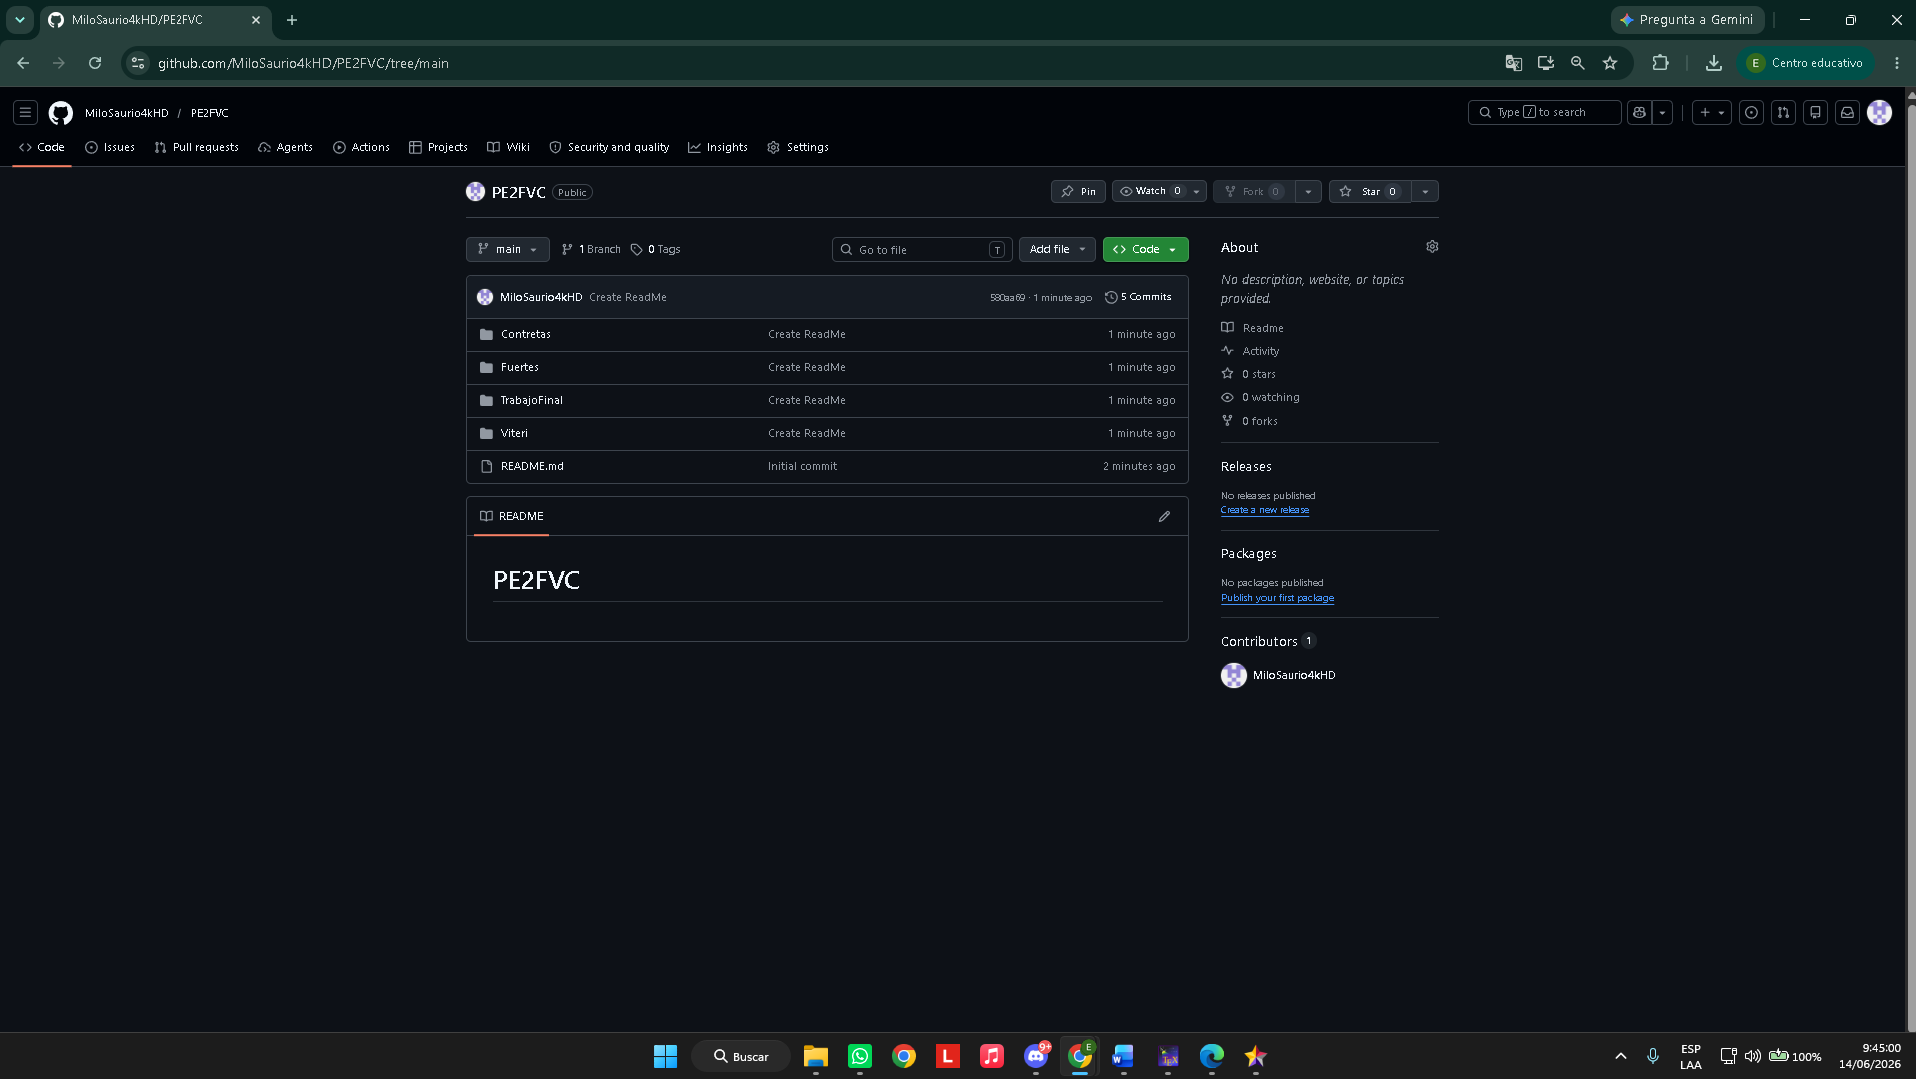
\includegraphics[width=\textwidth]{repositorio.png}}
	\caption{Repositorio del informe de la Práctica Experimental 2}
	\label{fig:repositorio-github}
\end{figure}

\begin{figure}[H]
	\centering
	\fbox{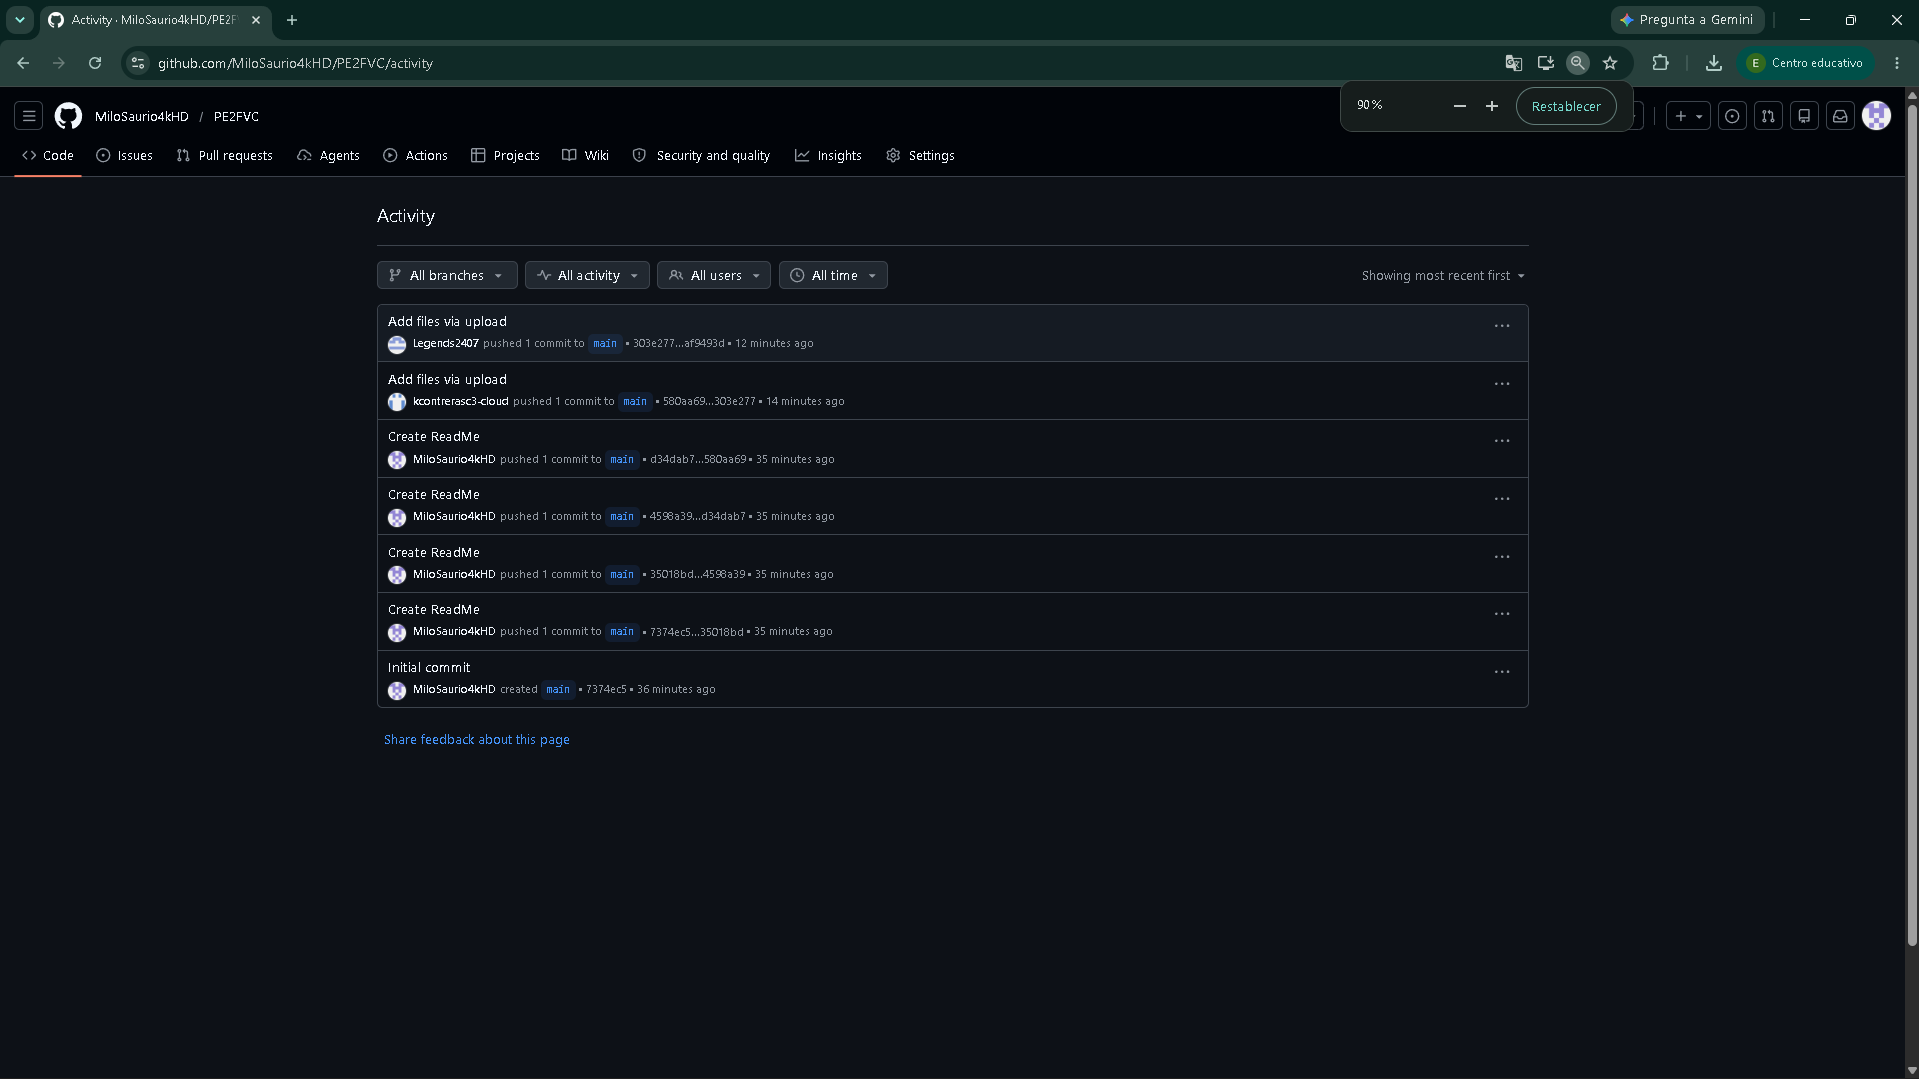
\includegraphics[width=\textwidth]{commits.png}}
	\caption{Commits al repositorio del informe de Práctica Experimental 2}
	\label{fig:commit-github}
\end{figure}

\end{document}
